\documentclass[twoside]{book}

% Packages required by doxygen
\usepackage{calc}
\usepackage{doxygen}
\usepackage{graphicx}
\usepackage[utf8]{inputenc}
\usepackage{makeidx}
\usepackage{multicol}
\usepackage{multirow}
\usepackage{textcomp}
\usepackage[table]{xcolor}

% Font selection
\usepackage[T1]{fontenc}
\usepackage{mathptmx}
\usepackage[scaled=.90]{helvet}
\usepackage{courier}
\usepackage{amssymb}
\usepackage{sectsty}
\renewcommand{\familydefault}{\sfdefault}
\allsectionsfont{%
  \fontseries{bc}\selectfont%
  \color{darkgray}%
}
\renewcommand{\DoxyLabelFont}{%
  \fontseries{bc}\selectfont%
  \color{darkgray}%
}

% Page & text layout
\usepackage{geometry}
\geometry{%
  a4paper,%
  top=2.5cm,%
  bottom=2.5cm,%
  left=2.5cm,%
  right=2.5cm%
}
\tolerance=750
\hfuzz=15pt
\hbadness=750
\setlength{\emergencystretch}{15pt}
\setlength{\parindent}{0cm}
\setlength{\parskip}{0.2cm}
\makeatletter
\renewcommand{\paragraph}{%
  \@startsection{paragraph}{4}{0ex}{-1.0ex}{1.0ex}{%
    \normalfont\normalsize\bfseries\SS@parafont%
  }%
}
\renewcommand{\subparagraph}{%
  \@startsection{subparagraph}{5}{0ex}{-1.0ex}{1.0ex}{%
    \normalfont\normalsize\bfseries\SS@subparafont%
  }%
}
\makeatother

% Headers & footers
\usepackage{fancyhdr}
\pagestyle{fancyplain}
\fancyhead[LE]{\fancyplain{}{\bfseries\thepage}}
\fancyhead[CE]{\fancyplain{}{}}
\fancyhead[RE]{\fancyplain{}{\bfseries\leftmark}}
\fancyhead[LO]{\fancyplain{}{\bfseries\rightmark}}
\fancyhead[CO]{\fancyplain{}{}}
\fancyhead[RO]{\fancyplain{}{\bfseries\thepage}}
\fancyfoot[LE]{\fancyplain{}{}}
\fancyfoot[CE]{\fancyplain{}{}}
\fancyfoot[RE]{\fancyplain{}{\bfseries\scriptsize Generated on Mon Oct 12 2015 23\-:36\-:25 for L\-I\-F\-T -\/ Lift Is not a Framework or Toolkit by Doxygen }}
\fancyfoot[LO]{\fancyplain{}{\bfseries\scriptsize Generated on Mon Oct 12 2015 23\-:36\-:25 for L\-I\-F\-T -\/ Lift Is not a Framework or Toolkit by Doxygen }}
\fancyfoot[CO]{\fancyplain{}{}}
\fancyfoot[RO]{\fancyplain{}{}}
\renewcommand{\footrulewidth}{0.4pt}
\renewcommand{\chaptermark}[1]{%
  \markboth{#1}{}%
}
\renewcommand{\sectionmark}[1]{%
  \markright{\thesection\ #1}%
}

% Indices & bibliography
\usepackage{natbib}
\usepackage[titles]{tocloft}
\setcounter{tocdepth}{3}
\setcounter{secnumdepth}{5}
\makeindex

% Hyperlinks (required, but should be loaded last)
\usepackage{ifpdf}
\ifpdf
  \usepackage[pdftex,pagebackref=true]{hyperref}
\else
  \usepackage[ps2pdf,pagebackref=true]{hyperref}
\fi
\hypersetup{%
  colorlinks=true,%
  linkcolor=blue,%
  citecolor=blue,%
  unicode%
}

% Custom commands
\newcommand{\clearemptydoublepage}{%
  \newpage{\pagestyle{empty}\cleardoublepage}%
}


%===== C O N T E N T S =====

\begin{document}

% Titlepage & ToC
\hypersetup{pageanchor=false}
\pagenumbering{roman}
\begin{titlepage}
\vspace*{7cm}
\begin{center}%
{\Large L\-I\-F\-T -\/ Lift Is not a Framework or Toolkit }\\
\vspace*{1cm}
{\large Generated by Doxygen 1.8.6}\\
\vspace*{0.5cm}
{\small Mon Oct 12 2015 23:36:25}\\
\end{center}
\end{titlepage}
\clearemptydoublepage
\tableofcontents
\clearemptydoublepage
\pagenumbering{arabic}
\hypersetup{pageanchor=true}

%--- Begin generated contents ---
\chapter{L\-I\-F\-T}
\label{index}\hypertarget{index}{}L\-I\-F\-T is a collectiong of useful C modules. It isn't a framework or a Toolkit. Most modules are either self-\/sufficient (depend only on parts of C standard library, or, in some cases, parts of standard library for a given system (P\-O\-S\-I\-X, Windows...)), or depend on a few other L\-I\-F\-T modules.

For a reasonably type-\/safe realloc for arrays (and, in most cases you use realloc for arrays), check out \hyperlink{lift__arealloc_8h}{lift\-\_\-arealloc.\-h}.

For a reasonably type-\/safe free that also N\-U\-L\-L-\/ifies the pointer, check out \hyperlink{lift__free__and__null_8h}{lift\-\_\-free\-\_\-and\-\_\-null.\-h}.

For a reasonably type-\/safe and efficient generic vector, with an interface inspired by C++ S\-T\-L, check out \hyperlink{lift__vec_8h}{lift\-\_\-vec.\-h}.

For a minimalistic, type-\/safe and efficient generic list, with interface having no resemblense of C++ S\-T\-L, check out \hyperlink{lift__list_8h}{lift\-\_\-list.\-h}. 
\chapter{lift-\/c}
\label{md_README}
\hypertarget{md_README}{}
This is a bunch of useful C modules. The name of this kind-\/of-\/library, \char`\"{}\-L\-I\-F\-T\char`\"{}, can be interpreted as a recursive acronym\-: Lift Is not a Framework or a Toolkit (a bunch of useful C modules).

Also, it is a slight pun on a well-\/known C++ library. This is C, we don't need a {\itshape boost} we just need a {\itshape lift}. \-:)

\subsection*{What is there}

Well, there is the \char`\"{}master\char`\"{} include file {\ttfamily \hyperlink{lift_8h}{lift.\-h}}, but, in most cases, you should just include the header of the module that you need. 
\chapter{Todo List}
\label{todo}
\hypertarget{todo}{}

\begin{DoxyRefList}
\item[\label{todo__todo000001}%
\hypertarget{todo__todo000001}{}%
Global \hyperlink{lift__vec_8h_a89038108b54f4ae2ca515776edc3b8ea}{lift\-\_\-vec\-\_\-resize} (var, newsize)]This doesn't handle all cases yet 
\end{DoxyRefList}
\chapter{File Index}
\section{File List}
Here is a list of all documented files with brief descriptions\-:\begin{DoxyCompactList}
\item\contentsline{section}{\hyperlink{lift_8h}{lift.\-h} }{\pageref{lift_8h}}{}
\item\contentsline{section}{\hyperlink{lift__arealloc_8h}{lift\-\_\-arealloc.\-h} \\*Safe alternative for realloc() for arrays }{\pageref{lift__arealloc_8h}}{}
\item\contentsline{section}{\hyperlink{lift__free__and__null_8h}{lift\-\_\-free\-\_\-and\-\_\-null.\-h} \\*A safer alternative to free() }{\pageref{lift__free__and__null_8h}}{}
\item\contentsline{section}{\hyperlink{lift__vec_8h}{lift\-\_\-vec.\-h} \\*A vector generic type for C }{\pageref{lift__vec_8h}}{}
\end{DoxyCompactList}

\chapter{File Documentation}
\hypertarget{lift_8h}{\section{lift.\-h File Reference}
\label{lift_8h}\index{lift.\-h@{lift.\-h}}
}
{\ttfamily \#include \char`\"{}lift\-\_\-arealloc.\-h\char`\"{}}\\*
Include dependency graph for lift.\-h\-:\nopagebreak
\begin{figure}[H]
\begin{center}
\leavevmode
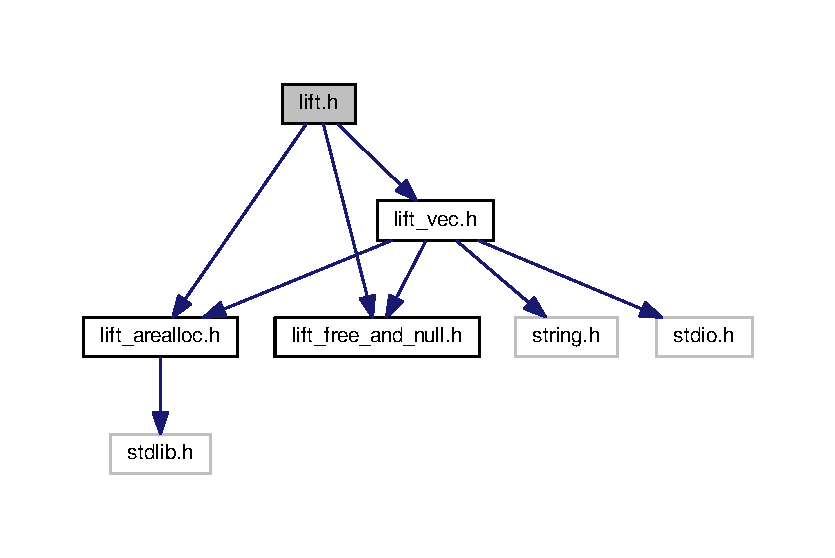
\includegraphics[width=154pt]{lift_8h__incl}
\end{center}
\end{figure}

\hypertarget{lift__arealloc_8h}{\section{lift\-\_\-arealloc.\-h File Reference}
\label{lift__arealloc_8h}\index{lift\-\_\-arealloc.\-h@{lift\-\_\-arealloc.\-h}}
}


Safe alternative for realloc() for arrays.  


{\ttfamily \#include $<$stdlib.\-h$>$}\\*
Include dependency graph for lift\-\_\-arealloc.\-h\-:\nopagebreak
\begin{figure}[H]
\begin{center}
\leavevmode
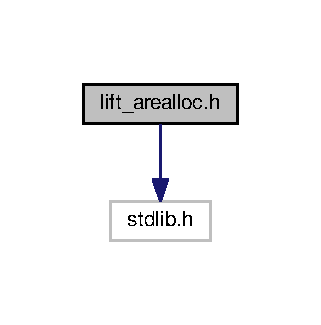
\includegraphics[width=154pt]{lift__arealloc_8h__incl}
\end{center}
\end{figure}
This graph shows which files directly or indirectly include this file\-:\nopagebreak
\begin{figure}[H]
\begin{center}
\leavevmode
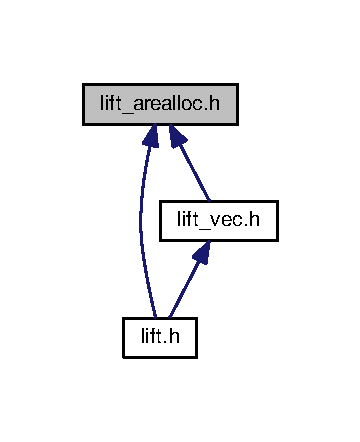
\includegraphics[width=189pt]{lift__arealloc_8h__dep__incl}
\end{center}
\end{figure}
\subsection*{Macros}
\begin{DoxyCompactItemize}
\item 
\#define \hyperlink{lift__arealloc_8h_aa29066af0304aa4445b7e13ccff595de}{lift\-\_\-arealloc}(ptr, members)~\hyperlink{lift__arealloc_8h_a2193a6bf115f8542b19f0225cfb6a306}{lift\-\_\-arealloc\-\_\-implementation}(\&(ptr),(members), sizeof $\ast$(ptr))
\begin{DoxyCompactList}\small\item\em This macro makes lif\-\_\-arealloc\-\_\-implementation() a lot easier to use and less error prone. \end{DoxyCompactList}\end{DoxyCompactItemize}
\subsection*{Functions}
\begin{DoxyCompactItemize}
\item 
void $\ast$ \hyperlink{lift__arealloc_8h_a2193a6bf115f8542b19f0225cfb6a306}{lift\-\_\-arealloc\-\_\-implementation} (void $\ast$ptrptr, size\-\_\-t members, size\-\_\-t size)
\begin{DoxyCompactList}\small\item\em A safe alternative to realloc() for arrays. \end{DoxyCompactList}\end{DoxyCompactItemize}


\subsection{Detailed Description}
Safe alternative for realloc() for arrays. Part of L\-I\-F\-T, but can be used on its own -\/ doesn't depend on anything from L\-I\-F\-T. \begin{DoxyAuthor}{Author}
Srdjan Veljkovic 
\end{DoxyAuthor}
\begin{DoxyCopyright}{Copyright}
M\-I\-T License 
\end{DoxyCopyright}


\subsection{Macro Definition Documentation}
\hypertarget{lift__arealloc_8h_aa29066af0304aa4445b7e13ccff595de}{\index{lift\-\_\-arealloc.\-h@{lift\-\_\-arealloc.\-h}!lift\-\_\-arealloc@{lift\-\_\-arealloc}}
\index{lift\-\_\-arealloc@{lift\-\_\-arealloc}!lift_arealloc.h@{lift\-\_\-arealloc.\-h}}
\subsubsection[{lift\-\_\-arealloc}]{\setlength{\rightskip}{0pt plus 5cm}\#define lift\-\_\-arealloc(
\begin{DoxyParamCaption}
\item[{}]{ptr, }
\item[{}]{members}
\end{DoxyParamCaption}
)~{\bf lift\-\_\-arealloc\-\_\-implementation}(\&(ptr),(members), sizeof $\ast$(ptr))}}\label{lift__arealloc_8h_aa29066af0304aa4445b7e13ccff595de}


This macro makes lif\-\_\-arealloc\-\_\-implementation() a lot easier to use and less error prone. 

It is a {\itshape good} macro, as it is very simple and doesn't evaluate its arguments more than once.

We fix two usability issues\-:
\begin{DoxyEnumerate}
\item You may pass a pointer (to a value) instead of a pointer to pointer
\item You may pass a wrong (element) size
\end{DoxyEnumerate}

Here we accept a pointer, and you can't pass a value. You can, of course pass a pointer to pointer, but, that may be valid input, so we can't reject that.

The size of an element is deduced to be {\ttfamily sizeof $\ast$ptr}.


\begin{DoxyParams}{Parameters}
{\em ptr} & The pointer to reallocate -\/ it will be changed \char`\"{}in place\char`\"{}, if need be. \\
\hline
{\em members} & The number of members of the new array \\
\hline
\end{DoxyParams}
\begin{DoxyReturn}{Returns}
Pointer to the new array or N\-U\-L\-L on failure to (re)allocate 
\end{DoxyReturn}
\begin{Desc}
\item[Examples\-: ]\par
\hyperlink{lift_arealloc_example_8c-example}{lift\-\_\-arealloc\-\_\-example.\-c}.\end{Desc}


\subsection{Function Documentation}
\hypertarget{lift__arealloc_8h_a2193a6bf115f8542b19f0225cfb6a306}{\index{lift\-\_\-arealloc.\-h@{lift\-\_\-arealloc.\-h}!lift\-\_\-arealloc\-\_\-implementation@{lift\-\_\-arealloc\-\_\-implementation}}
\index{lift\-\_\-arealloc\-\_\-implementation@{lift\-\_\-arealloc\-\_\-implementation}!lift_arealloc.h@{lift\-\_\-arealloc.\-h}}
\subsubsection[{lift\-\_\-arealloc\-\_\-implementation}]{\setlength{\rightskip}{0pt plus 5cm}void$\ast$ lift\-\_\-arealloc\-\_\-implementation (
\begin{DoxyParamCaption}
\item[{void $\ast$}]{ptrptr, }
\item[{size\-\_\-t}]{members, }
\item[{size\-\_\-t}]{size}
\end{DoxyParamCaption}
)}}\label{lift__arealloc_8h_a2193a6bf115f8542b19f0225cfb6a306}


A safe alternative to realloc() for arrays. 

It avoids the problems of overflow ({\ttfamily members} $\ast$  may overflow) and \char`\"{}leaking\char`\"{} the previously allocated memory in case of failure. In case you're not aware of it, here is the offending code\-: \begin{DoxyVerb}char *s = malloc(100);
s = realloc(s, 200);
\end{DoxyVerb}


If realloc() fails, {\ttfamily s} will now be N\-U\-L\-L, and previously malloc()-\/ ated memory is leaked, there is no way to free it now.

The only problem that \hyperlink{lift__arealloc_8h_aa29066af0304aa4445b7e13ccff595de}{lift\-\_\-arealloc()} doesn't solve is that passing an invalid pointer (not N\-U\-L\-L or \char`\"{}really\char`\"{} allocated) results in undefined behavior.

\begin{DoxyWarning}{Warning}
Don't forget to pass the address of your pointer, rather than the pointer itself, even though the formal parameter type for  is {\ttfamily void$\ast$}.
\end{DoxyWarning}
So, to fix the realloc() problem cited above, we would\-: \begin{DoxyVerb}char *s = malloc(100);
if (NULL == lift_arealloc(&s, 200, sizeof(char)) {
    // handle reallocation failure, but `s` stayed the same
}
\end{DoxyVerb}


\begin{DoxyNote}{Note}
The downside is that may simply forget to pass the address of your pointer, and pass the pointer itself, and there is no way that we can detect that. Declaring {\ttfamily ptrptr} to be a {\ttfamily void$\ast$$\ast$} would have actually been worse, as that would require cast if you want to avoid warnings (or even errors) for passing a pointer to, say, {\ttfamily int$\ast$}, instead of to {\ttfamily void$\ast$}. So, passing something like {\ttfamily 3}, because you cast it to {\ttfamily void$\ast$$\ast$} would not be detected.
\end{DoxyNote}
To help with these usability issues, you should probably use \hyperlink{lift__arealloc_8h_aa29066af0304aa4445b7e13ccff595de}{lift\-\_\-arealloc} macro instead of this function.

\begin{DoxyRemark}{Remarks}
On detecting overflow or any other invalid usage, it will {\itshape not} call realloc and will return N\-U\-L\-L and set {\ttfamily errno} to E\-R\-A\-N\-G\-E. If realloc() returns N\-U\-L\-L, {\ttfamily ptrptr} will not be changed. Otherwise, the result of realloc() will be written to {\ttfamily $\ast$ptrptr}.
\end{DoxyRemark}

\begin{DoxyParams}[1]{Parameters}
\mbox{\tt in,out}  & {\em ptrptr} & Pointer to pointer to be reallocated. N\-U\-L\-L is invalid. If not N\-U\-L\-L, and other checks pass, {\ttfamily $\ast$ptrptr} will passed to realloc().\\
\hline
\mbox{\tt in}  & {\em members} & The number of members of the new array. If the result of multiply with {\ttfamily size} doesn't overflow, that result will be passed to realloc(). Also, if it or  is 0, the function may fail.\\
\hline
\mbox{\tt in}  & {\em size} & Size of a member of the new array. If the result of multiply with {\ttfamily members} doesn't overflow, that result will be passed to realloc(). Also, if it or  is 0, the function may fail.\\
\hline
\end{DoxyParams}
\begin{DoxyReturn}{Returns}
On internal or realloc() failure, will return N\-U\-L\-L. Otherwise, will return the result of realloc(). 
\end{DoxyReturn}
\begin{Desc}
\item[Examples\-: ]\par
\hyperlink{lift_arealloc_example_8c-example}{lift\-\_\-arealloc\-\_\-example.\-c}.\end{Desc}

\hypertarget{lift__free__and__null_8h}{\section{lift\-\_\-free\-\_\-and\-\_\-null.\-h File Reference}
\label{lift__free__and__null_8h}\index{lift\-\_\-free\-\_\-and\-\_\-null.\-h@{lift\-\_\-free\-\_\-and\-\_\-null.\-h}}
}


A safer alternative to free().  


This graph shows which files directly or indirectly include this file\-:
\nopagebreak
\begin{figure}[H]
\begin{center}
\leavevmode
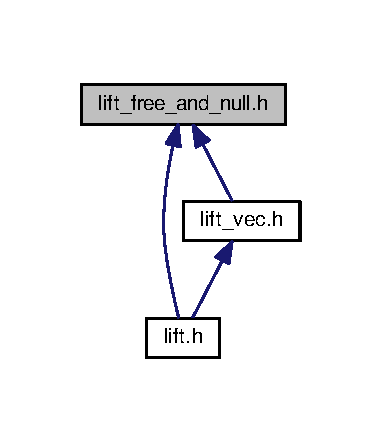
\includegraphics[width=184pt]{lift__free__and__null_8h__dep__incl}
\end{center}
\end{figure}
\subsection*{Macros}
\begin{DoxyCompactItemize}
\item 
\#define \hyperlink{lift__free__and__null_8h_ae429d1e4d6d8ae834f8174d6cf0b9e10}{lift\-\_\-nfree}(ptr)~\hyperlink{lift__free__and__null_8h_a873930b05bedfabc4dadf6df93a88428}{lift\-\_\-free\-\_\-and\-\_\-null}(\&(ptr)), sizeof $\ast$(ptr)
\begin{DoxyCompactList}\small\item\em This macro solves the usability problem with \hyperlink{lift__free__and__null_8h_a873930b05bedfabc4dadf6df93a88428}{lift\-\_\-free\-\_\-and\-\_\-null()}. \end{DoxyCompactList}\end{DoxyCompactItemize}
\subsection*{Functions}
\begin{DoxyCompactItemize}
\item 
void \hyperlink{lift__free__and__null_8h_a873930b05bedfabc4dadf6df93a88428}{lift\-\_\-free\-\_\-and\-\_\-null} (void $\ast$ptrptr)
\begin{DoxyCompactList}\small\item\em An alternative / wrapper to free(). \end{DoxyCompactList}\end{DoxyCompactItemize}


\subsection{Detailed Description}
A safer alternative to free(). \begin{DoxyAuthor}{Author}
Srdjan Veljkovic 
\end{DoxyAuthor}
\begin{DoxyCopyright}{Copyright}
M\-I\-T license 
\end{DoxyCopyright}


\subsection{Macro Definition Documentation}
\hypertarget{lift__free__and__null_8h_ae429d1e4d6d8ae834f8174d6cf0b9e10}{\index{lift\-\_\-free\-\_\-and\-\_\-null.\-h@{lift\-\_\-free\-\_\-and\-\_\-null.\-h}!lift\-\_\-nfree@{lift\-\_\-nfree}}
\index{lift\-\_\-nfree@{lift\-\_\-nfree}!lift_free_and_null.h@{lift\-\_\-free\-\_\-and\-\_\-null.\-h}}
\subsubsection[{lift\-\_\-nfree}]{\setlength{\rightskip}{0pt plus 5cm}\#define lift\-\_\-nfree(
\begin{DoxyParamCaption}
\item[{}]{ptr}
\end{DoxyParamCaption}
)~{\bf lift\-\_\-free\-\_\-and\-\_\-null}(\&(ptr)), sizeof $\ast$(ptr)}}\label{lift__free__and__null_8h_ae429d1e4d6d8ae834f8174d6cf0b9e10}


This macro solves the usability problem with \hyperlink{lift__free__and__null_8h_a873930b05bedfabc4dadf6df93a88428}{lift\-\_\-free\-\_\-and\-\_\-null()}. 

It is a {\itshape good} macro, as it is simple and does not evaluate its argument more than once.

Here we expect a pointer and you can't pass a variable. Of course, you may pass a pointer to pointer, but that may be valid input.

There is an additional check -\/ you can't pass a void pointer. That means that some strange, but valid code, will not compile. If you have such code, use \hyperlink{lift__free__and__null_8h_a873930b05bedfabc4dadf6df93a88428}{lift\-\_\-free\-\_\-and\-\_\-null()}, but be careful.


\begin{DoxyParams}{Parameters}
{\em ptr} & The pointer to free (previously allocated by malloc() or realloc()). It will be set to N\-U\-L\-L \char`\"{}in place\char`\"{} \\
\hline
\end{DoxyParams}
\begin{DoxyReturn}{Returns}
The size of what the {\ttfamily ptr} points to 
\end{DoxyReturn}
\begin{Desc}
\item[Examples\-: ]\par
\hyperlink{lift_free_and_null_example_8c-example}{lift\-\_\-free\-\_\-and\-\_\-null\-\_\-example.\-c}.\end{Desc}


\subsection{Function Documentation}
\hypertarget{lift__free__and__null_8h_a873930b05bedfabc4dadf6df93a88428}{\index{lift\-\_\-free\-\_\-and\-\_\-null.\-h@{lift\-\_\-free\-\_\-and\-\_\-null.\-h}!lift\-\_\-free\-\_\-and\-\_\-null@{lift\-\_\-free\-\_\-and\-\_\-null}}
\index{lift\-\_\-free\-\_\-and\-\_\-null@{lift\-\_\-free\-\_\-and\-\_\-null}!lift_free_and_null.h@{lift\-\_\-free\-\_\-and\-\_\-null.\-h}}
\subsubsection[{lift\-\_\-free\-\_\-and\-\_\-null}]{\setlength{\rightskip}{0pt plus 5cm}void lift\-\_\-free\-\_\-and\-\_\-null (
\begin{DoxyParamCaption}
\item[{void $\ast$}]{ptrptr}
\end{DoxyParamCaption}
)}}\label{lift__free__and__null_8h_a873930b05bedfabc4dadf6df93a88428}


An alternative / wrapper to free(). 

It will N\-U\-L\-L the pointer, not just free() it. Thus, you will not have a dangling pointer.

Passing N\-U\-L\-L or a pointer to N\-U\-L\-L (pointer) will simply be ignored. Otherwise, free() will be called on {\ttfamily $\ast$ptrptr} and then it will be N\-U\-L\-L-\/ed.

\begin{DoxyWarning}{Warning}
You must pass the address of your pointer, not the pointer itself. Since {\ttfamily ptrptr} is of {\ttfamily void$\ast$}, it will not detect if you pass the pointer, and we shall have undefined behavior.
\end{DoxyWarning}
\begin{DoxyRemark}{Remarks}
The advantage of this function versus a pure macro implementation is that we avoid the problem of multiple evaluation in the macro. That should make it easier to find bugs with not passing address of a pointer (but the pointer itself).
\end{DoxyRemark}
We provida macro wrapper in \hyperlink{lift__free__and__null_8h_ae429d1e4d6d8ae834f8174d6cf0b9e10}{lift\-\_\-nfree}, that solves this usability problem.

\begin{DoxyRemark}{Remarks}
Declaring {\ttfamily ptrptr} to be of {\ttfamily void $\ast$$\ast$} type would be much worse, as to silence warnings (or maybe errors) one would need to cast to {\ttfamily void$\ast$$\ast$} always, which would enable passing {\itshape anything}.
\end{DoxyRemark}

\begin{DoxyParams}[1]{Parameters}
\mbox{\tt in,out}  & {\em ptrptr} & Pointer to the pointer to free and N\-U\-L\-L \\
\hline
\end{DoxyParams}
\begin{Desc}
\item[Examples\-: ]\par
\hyperlink{lift_free_and_null_example_8c-example}{lift\-\_\-free\-\_\-and\-\_\-null\-\_\-example.\-c}.\end{Desc}

\hypertarget{lift__vec_8h}{\section{lift\-\_\-vec.\-h File Reference}
\label{lift__vec_8h}\index{lift\-\_\-vec.\-h@{lift\-\_\-vec.\-h}}
}


A vector generic type for C.  


{\ttfamily \#include \char`\"{}lift\-\_\-arealloc.\-h\char`\"{}}\\*
{\ttfamily \#include \char`\"{}lift\-\_\-free\-\_\-and\-\_\-null.\-h\char`\"{}}\\*
{\ttfamily \#include $<$string.\-h$>$}\\*
{\ttfamily \#include $<$stdio.\-h$>$}\\*
Include dependency graph for lift\-\_\-vec.\-h\-:\nopagebreak
\begin{figure}[H]
\begin{center}
\leavevmode
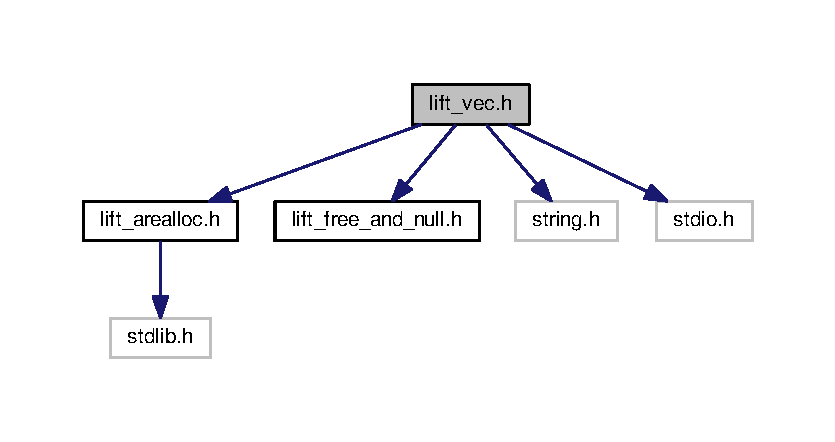
\includegraphics[width=350pt]{lift__vec_8h__incl}
\end{center}
\end{figure}
\subsection*{Macros}
\begin{DoxyCompactItemize}
\item 
\#define \hyperlink{lift__vec_8h_a953ac441707c2affe21bcd56a639c502}{L\-I\-F\-T\-\_\-\-D\-E\-C\-L\-\_\-\-V\-E\-C}(typ)~struct \{ unsigned n; unsigned c; typ $\ast$p; \}
\begin{DoxyCompactList}\small\item\em Declare a vector for the given type {\ttfamily typ}. \end{DoxyCompactList}\item 
\#define \hyperlink{lift__vec_8h_a5f062efdf1ed0cb5bd5ea58c2e3c380d}{L\-I\-F\-T\-\_\-\-V\-E\-C\-\_\-\-V\-A\-R}(typ, var)~L\-I\-F\-T\-\_\-\-D\-E\-C\-L\-\_\-\-V\-E\-C\-T(typ) =  \{ 0, 0, N\-U\-L\-L \}
\begin{DoxyCompactList}\small\item\em Declare a variable of the vector of type {\ttfamily typ}, with the name (symbol) {\ttfamily var}. \end{DoxyCompactList}\item 
\hypertarget{lift__vec_8h_ad9081bbf2d35f6e47bfac8b758b7ea48}{\#define {\bfseries L\-I\-F\-T\-\_\-\-V\-E\-C\-\_\-\-I\-N\-I\-T}(var)~memset(\&(var), 0, sizeof (var))}\label{lift__vec_8h_ad9081bbf2d35f6e47bfac8b758b7ea48}

\item 
\#define \hyperlink{lift__vec_8h_a09e49321f68f213ed563b36026507904}{lift\-\_\-vec\-\_\-begin}(var)~((var).p)
\begin{DoxyCompactList}\small\item\em Gives an iterator (pointer, really) to the begining of the vector {\ttfamily var}. \end{DoxyCompactList}\item 
\#define \hyperlink{lift__vec_8h_a3e99cd489d53306dc19917e5ad400ba8}{lift\-\_\-vec\-\_\-end}(var)~((var).p + (var).n)
\begin{DoxyCompactList}\small\item\em Gives an iterator (pointer, really) to the end of the vector {\ttfamily var}. \end{DoxyCompactList}\item 
\hypertarget{lift__vec_8h_ab6b2d109dfea9c0f2f186c9add41e669}{\#define {\bfseries L\-I\-F\-T\-\_\-\-V\-E\-C\-\_\-\-V\-A\-L\-I\-D\-\_\-\-I\-T\-E\-R\-A\-T\-O\-R}(var, iter)~(((iter) $>$= \hyperlink{lift__vec_8h_a09e49321f68f213ed563b36026507904}{lift\-\_\-vec\-\_\-begin}(var)) \&\& (((iter) $<$= \hyperlink{lift__vec_8h_a3e99cd489d53306dc19917e5ad400ba8}{lift\-\_\-vec\-\_\-end}(var))))}\label{lift__vec_8h_ab6b2d109dfea9c0f2f186c9add41e669}

\item 
\hypertarget{lift__vec_8h_a460948ccbbb7690e71a9fdb1051b97a8}{\#define {\bfseries L\-I\-F\-T\-\_\-\-V\-E\-C\-\_\-\-S\-A\-F\-E\-\_\-\-I\-T\-E\-R\-A\-T\-O\-R}(var, iter)~(((iter) $>$= \hyperlink{lift__vec_8h_a09e49321f68f213ed563b36026507904}{lift\-\_\-vec\-\_\-begin}(var)) \&\& (((iter) $<$ \hyperlink{lift__vec_8h_a3e99cd489d53306dc19917e5ad400ba8}{lift\-\_\-vec\-\_\-end}(var))))}\label{lift__vec_8h_a460948ccbbb7690e71a9fdb1051b97a8}

\item 
\hypertarget{lift__vec_8h_aa95dcb31fe93ca880d8f94232a71f0a3}{\#define \hyperlink{lift__vec_8h_aa95dcb31fe93ca880d8f94232a71f0a3}{lift\-\_\-vec\-\_\-size}(var)~((var).n)}\label{lift__vec_8h_aa95dcb31fe93ca880d8f94232a71f0a3}

\begin{DoxyCompactList}\small\item\em Returns the number of elements in the vector {\ttfamily var}. \end{DoxyCompactList}\item 
\#define \hyperlink{lift__vec_8h_a89038108b54f4ae2ca515776edc3b8ea}{lift\-\_\-vec\-\_\-resize}(var, newsize)
\begin{DoxyCompactList}\small\item\em Resizes the vector {\ttfamily var} to have {\ttfamily newsize} elements. \end{DoxyCompactList}\item 
\hypertarget{lift__vec_8h_a80ec213390d3900ec81e15c1b0932f24}{\#define \hyperlink{lift__vec_8h_a80ec213390d3900ec81e15c1b0932f24}{lift\-\_\-vec\-\_\-capacity}(var)~((var).c)}\label{lift__vec_8h_a80ec213390d3900ec81e15c1b0932f24}

\begin{DoxyCompactList}\small\item\em Returns the current capacity of the vectory {\ttfamily var}. \end{DoxyCompactList}\item 
\hypertarget{lift__vec_8h_a4d7e791410bec3b894b04ad7435816f0}{\#define \hyperlink{lift__vec_8h_a4d7e791410bec3b894b04ad7435816f0}{lift\-\_\-vec\-\_\-empty}(var)~(0 == (var).n)}\label{lift__vec_8h_a4d7e791410bec3b894b04ad7435816f0}

\begin{DoxyCompactList}\small\item\em Returns whether the vectory {\ttfamily var} is empty (has no elements) \end{DoxyCompactList}\item 
\#define \hyperlink{lift__vec_8h_a5946d0be6518dfbe8d315503aa213adc}{lift\-\_\-vec\-\_\-reserve}(var, newcap)
\begin{DoxyCompactList}\small\item\em Reserves the memory for vectory {\ttfamily var} to have place for {\ttfamily newcap} elements. \end{DoxyCompactList}\item 
\#define \hyperlink{lift__vec_8h_a2e13eb1aa433c210e93429d81d2ecd42}{lift\-\_\-vec\-\_\-push\-\_\-back}(var, val)
\begin{DoxyCompactList}\small\item\em Pushes the value {\ttfamily val} to the end of vector {\ttfamily var}, increasing the vector's size. \end{DoxyCompactList}\item 
\#define \hyperlink{lift__vec_8h_a83bc357f9b6ffd618f89af9eca3bf5df}{lift\-\_\-vec\-\_\-pop\-\_\-back}(var)
\begin{DoxyCompactList}\small\item\em Removes the last element of the vectory {\ttfamily var}, if the vector is not empty. \end{DoxyCompactList}\item 
\#define \hyperlink{lift__vec_8h_ac79c356c99fcb743ceb51e91f7fc3375}{lift\-\_\-vec\-\_\-insert}(var, pos, val)
\begin{DoxyCompactList}\small\item\em Inserts the value {\ttfamily val} into the vector {\ttfamily var} at iterator/position {\ttfamily pos}. \end{DoxyCompactList}\item 
\#define \hyperlink{lift__vec_8h_ab3ec35f976e8f95f2a341763a6599a8a}{lift\-\_\-vec\-\_\-erase}(var, pos)
\begin{DoxyCompactList}\small\item\em Erases the element of the vector {\ttfamily var} at iterator/position {\ttfamily pos}. \end{DoxyCompactList}\item 
\#define \hyperlink{lift__vec_8h_acf6d249b5825f99d1b9bf4cd42454cd3}{lift\-\_\-vec\-\_\-free}(var)~\hyperlink{lift__free__and__null_8h_ae429d1e4d6d8ae834f8174d6cf0b9e10}{lift\-\_\-nfree}((var).p), (var).n = (var).c = 0
\begin{DoxyCompactList}\small\item\em Once you're done with the vector, use this macro to free any resources (memory) that was allocated during its use. \end{DoxyCompactList}\item 
\#define \hyperlink{lift__vec_8h_a7d624f15bbaa9253611a44b406b4c0a0}{lift\-\_\-vec\-\_\-front}(var)~\hyperlink{lift__vec_8h_a3f85aaaa1f14453788b811ffcd3c37d4}{lift\-\_\-vec\-\_\-at}(var, 0)
\begin{DoxyCompactList}\small\item\em Allows you to set element at the front (beginning) of the vector. \end{DoxyCompactList}\item 
\hypertarget{lift__vec_8h_a204b51e518a7769c7eee86c4e40abd2a}{\#define \hyperlink{lift__vec_8h_a204b51e518a7769c7eee86c4e40abd2a}{lift\-\_\-vec\-\_\-front\-\_\-get}(var)~(\hyperlink{lift__vec_8h_a3f85aaaa1f14453788b811ffcd3c37d4}{lift\-\_\-vec\-\_\-at}(var, 0))}\label{lift__vec_8h_a204b51e518a7769c7eee86c4e40abd2a}

\begin{DoxyCompactList}\small\item\em Returns the element at the front (beginning) of the vector. \end{DoxyCompactList}\item 
\#define \hyperlink{lift__vec_8h_a1f806932d91c072afa1b16d4a933d3d0}{lift\-\_\-vec\-\_\-back}(var)~\hyperlink{lift__vec_8h_a3f85aaaa1f14453788b811ffcd3c37d4}{lift\-\_\-vec\-\_\-at}((var), (var).n-\/1)
\begin{DoxyCompactList}\small\item\em Allows you to set element at the back of the vector (last element). \end{DoxyCompactList}\item 
\hypertarget{lift__vec_8h_afe2326662ff61f6073ad1728558ba2d9}{\#define \hyperlink{lift__vec_8h_afe2326662ff61f6073ad1728558ba2d9}{lift\-\_\-vec\-\_\-back\-\_\-get}(var)~(\hyperlink{lift__vec_8h_a3f85aaaa1f14453788b811ffcd3c37d4}{lift\-\_\-vec\-\_\-at}(var, (var).n-\/1))}\label{lift__vec_8h_afe2326662ff61f6073ad1728558ba2d9}

\begin{DoxyCompactList}\small\item\em Returns the element at the front (beginning) of the vector. \end{DoxyCompactList}\item 
\hypertarget{lift__vec_8h_accab99ecc2bf68085f004fe81c822112}{\#define \hyperlink{lift__vec_8h_accab99ecc2bf68085f004fe81c822112}{lift\-\_\-vec\-\_\-data}(var)~(var).p}\label{lift__vec_8h_accab99ecc2bf68085f004fe81c822112}

\begin{DoxyCompactList}\small\item\em Returns the data (array pointer) of the vector {\ttfamily var}, which you can pass to some function that expects such things. \end{DoxyCompactList}\item 
\hypertarget{lift__vec_8h_a0086251626d7d199046365bfb574c4e2}{\#define \hyperlink{lift__vec_8h_a0086251626d7d199046365bfb574c4e2}{L\-I\-F\-T\-\_\-\-V\-E\-C\-\_\-\-V\-A\-L\-I\-D}(var)~((var).p != N\-U\-L\-L)}\label{lift__vec_8h_a0086251626d7d199046365bfb574c4e2}

\begin{DoxyCompactList}\small\item\em Returns whether the vector {\ttfamily var} is valid. \end{DoxyCompactList}\item 
\hypertarget{lift__vec_8h_a7ad8de6e820ee182d665d85f610032d2}{\#define \hyperlink{lift__vec_8h_a7ad8de6e820ee182d665d85f610032d2}{L\-I\-F\-T\-\_\-\-V\-E\-C\-\_\-\-S\-A\-F\-E}(var, idx)~(idx $<$ \hyperlink{lift__vec_8h_aa95dcb31fe93ca880d8f94232a71f0a3}{lift\-\_\-vec\-\_\-size}(var))}\label{lift__vec_8h_a7ad8de6e820ee182d665d85f610032d2}

\begin{DoxyCompactList}\small\item\em Returns whether it is safe to access the element at index {\ttfamily idx} of the vector {\ttfamily var}. \end{DoxyCompactList}\item 
\hypertarget{lift__vec_8h_a3f85aaaa1f14453788b811ffcd3c37d4}{\#define \hyperlink{lift__vec_8h_a3f85aaaa1f14453788b811ffcd3c37d4}{lift\-\_\-vec\-\_\-at}(var, idx)~assert(\hyperlink{lift__vec_8h_a7ad8de6e820ee182d665d85f610032d2}{L\-I\-F\-T\-\_\-\-V\-E\-C\-\_\-\-S\-A\-F\-E}(var,idx)), \hyperlink{lift__vec_8h_a09e49321f68f213ed563b36026507904}{lift\-\_\-vec\-\_\-begin}(var)\mbox{[}idx\mbox{]}}\label{lift__vec_8h_a3f85aaaa1f14453788b811ffcd3c37d4}

\begin{DoxyCompactList}\small\item\em Gives the element at index {\ttfamily idx} of the vector {\ttfamily var}, checking if it is safe to access it. \end{DoxyCompactList}\item 
\hypertarget{lift__vec_8h_aa141c82ad99aa01241f9f3bc33bf9987}{\#define \hyperlink{lift__vec_8h_aa141c82ad99aa01241f9f3bc33bf9987}{lift\-\_\-vec\-\_\-get}(var, idx)~(\hyperlink{lift__vec_8h_a3f85aaaa1f14453788b811ffcd3c37d4}{lift\-\_\-vec\-\_\-at}(var,idx))}\label{lift__vec_8h_aa141c82ad99aa01241f9f3bc33bf9987}

\begin{DoxyCompactList}\small\item\em Returns the element at index {\ttfamily idx} of the vector {\ttfamily var}, checking if it is safe to access it. \end{DoxyCompactList}\item 
\#define \hyperlink{lift__vec_8h_a328160cf98397947580f3854727c1f2a}{L\-I\-F\-T\-\_\-\-V\-E\-C\-\_\-\-F\-O\-R\-\_\-\-E\-A\-C\-H\-\_\-\-I\-D\-X}(idx, var)~for (idx = 0; idx $<$ \hyperlink{lift__vec_8h_aa95dcb31fe93ca880d8f94232a71f0a3}{lift\-\_\-vec\-\_\-size}(var); ++idx)
\begin{DoxyCompactList}\small\item\em A helper macro to execute a for-\/each loop on the vector {\ttfamily var}, accessing by the index {\ttfamily idx}. \end{DoxyCompactList}\item 
\#define \hyperlink{lift__vec_8h_ae51b80ad7deb1a897534ec12405568db}{L\-I\-F\-T\-\_\-\-V\-E\-C\-\_\-\-F\-O\-R\-\_\-\-E\-A\-C\-H\-\_\-\-I\-T\-E\-R}(it, var)~for (it = \hyperlink{lift__vec_8h_a09e49321f68f213ed563b36026507904}{lift\-\_\-vec\-\_\-begin}(var); it != \hyperlink{lift__vec_8h_a3e99cd489d53306dc19917e5ad400ba8}{lift\-\_\-vec\-\_\-end}(var); ++it)
\begin{DoxyCompactList}\small\item\em A helper macro to execute a for-\/each loop on the vector {\ttfamily var}, accessing by the iterator/pointer {\ttfamily it}. \end{DoxyCompactList}\item 
\#define \hyperlink{lift__vec_8h_a88b3bd2c4be95af37a75a6576b2ffafe}{lift\-\_\-vec\-\_\-find}(var, val, rslt)
\begin{DoxyCompactList}\small\item\em A helper macro to search for the value {\ttfamily val} in the vector {\ttfamily var}. \end{DoxyCompactList}\item 
\hypertarget{lift__vec_8h_ab4b8005f19e2530b27dc643cc32a3be4}{\#define \hyperlink{lift__vec_8h_ab4b8005f19e2530b27dc643cc32a3be4}{L\-I\-F\-T\-\_\-\-P\-R\-I\-N\-T\-F}(var)~printf(\char`\"{}'\char`\"{}\#var \char`\"{}' lift\-\_\-vec\-: size=\%d, capacity=\%d, data=\%p\textbackslash{}n\char`\"{}, (var).n, (var).c, (var).p)}\label{lift__vec_8h_ab4b8005f19e2530b27dc643cc32a3be4}

\begin{DoxyCompactList}\small\item\em A helper macro to printf-\/out the vector {\ttfamily var}. \end{DoxyCompactList}\end{DoxyCompactItemize}


\subsection{Detailed Description}
A vector generic type for C. It is modelled after the C++ (S\-T\-L) vector. It is a macro implementation, but some care was taken to make it as safe as possible\-:


\begin{DoxyItemize}
\item No variables are declared in the macros themselves
\item Most macros are expressions
\item There is a reasonable amount of checking done...
\item ...and most type errors will be caught, with maybe ugly compiler errors
\end{DoxyItemize}

The only significant problem with this implementation is that {\itshape a} lot of parameters in these macros a evaluated more than once. So, you have to be careful not to pass expressions with side effects.

\begin{DoxyAuthor}{Author}
Srdjan Veljkovic 
\end{DoxyAuthor}
\begin{DoxyCopyright}{Copyright}
M\-I\-T License 
\end{DoxyCopyright}


\subsection{Macro Definition Documentation}
\hypertarget{lift__vec_8h_a953ac441707c2affe21bcd56a639c502}{\index{lift\-\_\-vec.\-h@{lift\-\_\-vec.\-h}!L\-I\-F\-T\-\_\-\-D\-E\-C\-L\-\_\-\-V\-E\-C@{L\-I\-F\-T\-\_\-\-D\-E\-C\-L\-\_\-\-V\-E\-C}}
\index{L\-I\-F\-T\-\_\-\-D\-E\-C\-L\-\_\-\-V\-E\-C@{L\-I\-F\-T\-\_\-\-D\-E\-C\-L\-\_\-\-V\-E\-C}!lift_vec.h@{lift\-\_\-vec.\-h}}
\subsubsection[{L\-I\-F\-T\-\_\-\-D\-E\-C\-L\-\_\-\-V\-E\-C}]{\setlength{\rightskip}{0pt plus 5cm}\#define L\-I\-F\-T\-\_\-\-D\-E\-C\-L\-\_\-\-V\-E\-C(
\begin{DoxyParamCaption}
\item[{}]{typ}
\end{DoxyParamCaption}
)~struct \{ unsigned n; unsigned c; typ $\ast$p; \}}}\label{lift__vec_8h_a953ac441707c2affe21bcd56a639c502}


Declare a vector for the given type {\ttfamily typ}. 

A lot of the time you should {\ttfamily typedef} this. \begin{Desc}
\item[Examples\-: ]\par
\hyperlink{lift_vec_example_8c-example}{lift\-\_\-vec\-\_\-example.\-c}.\end{Desc}
\hypertarget{lift__vec_8h_a1f806932d91c072afa1b16d4a933d3d0}{\index{lift\-\_\-vec.\-h@{lift\-\_\-vec.\-h}!lift\-\_\-vec\-\_\-back@{lift\-\_\-vec\-\_\-back}}
\index{lift\-\_\-vec\-\_\-back@{lift\-\_\-vec\-\_\-back}!lift_vec.h@{lift\-\_\-vec.\-h}}
\subsubsection[{lift\-\_\-vec\-\_\-back}]{\setlength{\rightskip}{0pt plus 5cm}\#define lift\-\_\-vec\-\_\-back(
\begin{DoxyParamCaption}
\item[{}]{var}
\end{DoxyParamCaption}
)~{\bf lift\-\_\-vec\-\_\-at}((var), (var).n-\/1)}}\label{lift__vec_8h_a1f806932d91c072afa1b16d4a933d3d0}


Allows you to set element at the back of the vector (last element). 

Use like\-: {\ttfamily \hyperlink{lift__vec_8h_a3e99cd489d53306dc19917e5ad400ba8}{lift\-\_\-vec\-\_\-end(v)} = 43;}. \hypertarget{lift__vec_8h_a09e49321f68f213ed563b36026507904}{\index{lift\-\_\-vec.\-h@{lift\-\_\-vec.\-h}!lift\-\_\-vec\-\_\-begin@{lift\-\_\-vec\-\_\-begin}}
\index{lift\-\_\-vec\-\_\-begin@{lift\-\_\-vec\-\_\-begin}!lift_vec.h@{lift\-\_\-vec.\-h}}
\subsubsection[{lift\-\_\-vec\-\_\-begin}]{\setlength{\rightskip}{0pt plus 5cm}\#define lift\-\_\-vec\-\_\-begin(
\begin{DoxyParamCaption}
\item[{}]{var}
\end{DoxyParamCaption}
)~((var).p)}}\label{lift__vec_8h_a09e49321f68f213ed563b36026507904}


Gives an iterator (pointer, really) to the begining of the vector {\ttfamily var}. 

This is the first element if vector is not empty. If the vector is empty, the only guarantee is that \hyperlink{lift__vec_8h_a09e49321f68f213ed563b36026507904}{lift\-\_\-vec\-\_\-begin(v)} == \hyperlink{lift__vec_8h_a3e99cd489d53306dc19917e5ad400ba8}{lift\-\_\-vec\-\_\-end(v)}. \begin{Desc}
\item[Examples\-: ]\par
\hyperlink{lift_vec_example_8c-example}{lift\-\_\-vec\-\_\-example.\-c}.\end{Desc}
\hypertarget{lift__vec_8h_a3e99cd489d53306dc19917e5ad400ba8}{\index{lift\-\_\-vec.\-h@{lift\-\_\-vec.\-h}!lift\-\_\-vec\-\_\-end@{lift\-\_\-vec\-\_\-end}}
\index{lift\-\_\-vec\-\_\-end@{lift\-\_\-vec\-\_\-end}!lift_vec.h@{lift\-\_\-vec.\-h}}
\subsubsection[{lift\-\_\-vec\-\_\-end}]{\setlength{\rightskip}{0pt plus 5cm}\#define lift\-\_\-vec\-\_\-end(
\begin{DoxyParamCaption}
\item[{}]{var}
\end{DoxyParamCaption}
)~((var).p + (var).n)}}\label{lift__vec_8h_a3e99cd489d53306dc19917e5ad400ba8}


Gives an iterator (pointer, really) to the end of the vector {\ttfamily var}. 

This points to an element one past the last element of the vector, if vectory is not empty. If the vector is empty, the only guarantee is that \hyperlink{lift__vec_8h_a09e49321f68f213ed563b36026507904}{lift\-\_\-vec\-\_\-begin(v)} == \hyperlink{lift__vec_8h_a3e99cd489d53306dc19917e5ad400ba8}{lift\-\_\-vec\-\_\-end(v)}. \begin{Desc}
\item[Examples\-: ]\par
\hyperlink{lift_vec_example_8c-example}{lift\-\_\-vec\-\_\-example.\-c}.\end{Desc}
\hypertarget{lift__vec_8h_ab3ec35f976e8f95f2a341763a6599a8a}{\index{lift\-\_\-vec.\-h@{lift\-\_\-vec.\-h}!lift\-\_\-vec\-\_\-erase@{lift\-\_\-vec\-\_\-erase}}
\index{lift\-\_\-vec\-\_\-erase@{lift\-\_\-vec\-\_\-erase}!lift_vec.h@{lift\-\_\-vec.\-h}}
\subsubsection[{lift\-\_\-vec\-\_\-erase}]{\setlength{\rightskip}{0pt plus 5cm}\#define lift\-\_\-vec\-\_\-erase(
\begin{DoxyParamCaption}
\item[{}]{var, }
\item[{}]{pos}
\end{DoxyParamCaption}
)}}\label{lift__vec_8h_ab3ec35f976e8f95f2a341763a6599a8a}
{\bfseries Value\-:}
\begin{DoxyCode}
(LIFT\_VEC\_SAFE\_ITERATOR(var, pos) ?                                 \(\backslash\)
     (                                                                  \(\backslash\)
         memmove((pos), (pos) + 1, ((var).n - 1 - ((pos) - \hyperlink{lift__vec_8h_a09e49321f68f213ed563b36026507904}{lift\_vec\_begin}(var))) * \textcolor{keyword}{sizeof} *(
      var).p), \(\backslash\)
         --(var).n,                                                     \(\backslash\)
         (pos))                                                         \(\backslash\)
     : NULL                                                             \(\backslash\)
        )
\end{DoxyCode}


Erases the element of the vector {\ttfamily var} at iterator/position {\ttfamily pos}. 

The {\ttfamily pos} has to be a safe iterator -\/ meaning, it can't be the \char`\"{}end\char`\"{}. On success, decreases the size of the vector {\ttfamily var} and returns the iterator at which the value {\ttfamily val} was erased. On error, returns N\-U\-L\-L. \begin{Desc}
\item[Examples\-: ]\par
\hyperlink{lift_vec_example_8c-example}{lift\-\_\-vec\-\_\-example.\-c}.\end{Desc}
\hypertarget{lift__vec_8h_a88b3bd2c4be95af37a75a6576b2ffafe}{\index{lift\-\_\-vec.\-h@{lift\-\_\-vec.\-h}!lift\-\_\-vec\-\_\-find@{lift\-\_\-vec\-\_\-find}}
\index{lift\-\_\-vec\-\_\-find@{lift\-\_\-vec\-\_\-find}!lift_vec.h@{lift\-\_\-vec.\-h}}
\subsubsection[{lift\-\_\-vec\-\_\-find}]{\setlength{\rightskip}{0pt plus 5cm}\#define lift\-\_\-vec\-\_\-find(
\begin{DoxyParamCaption}
\item[{}]{var, }
\item[{}]{val, }
\item[{}]{rslt}
\end{DoxyParamCaption}
)}}\label{lift__vec_8h_a88b3bd2c4be95af37a75a6576b2ffafe}
{\bfseries Value\-:}
\begin{DoxyCode}
\textcolor{keywordflow}{for} (rslt = \hyperlink{lift__vec_8h_a09e49321f68f213ed563b36026507904}{lift\_vec\_begin}(var); rslt != \hyperlink{lift__vec_8h_a3e99cd489d53306dc19917e5ad400ba8}{lift\_vec\_end}(var); ++rslt) \{ \(\backslash\)
        if (*rslt == (val)) \{                                           \(\backslash\)
            break;                                                      \(\backslash\)
        \}                                                               \(\backslash\)
    \}
\end{DoxyCode}


A helper macro to search for the value {\ttfamily val} in the vector {\ttfamily var}. 

The result will be stored in the iterator/pointer {\ttfamily rslt}, that you must provide. On success, it will give a safe iterator/position at which the given value was found. On failure, it will give the end iterator. \begin{Desc}
\item[Examples\-: ]\par
\hyperlink{lift_vec_example_8c-example}{lift\-\_\-vec\-\_\-example.\-c}.\end{Desc}
\hypertarget{lift__vec_8h_a328160cf98397947580f3854727c1f2a}{\index{lift\-\_\-vec.\-h@{lift\-\_\-vec.\-h}!L\-I\-F\-T\-\_\-\-V\-E\-C\-\_\-\-F\-O\-R\-\_\-\-E\-A\-C\-H\-\_\-\-I\-D\-X@{L\-I\-F\-T\-\_\-\-V\-E\-C\-\_\-\-F\-O\-R\-\_\-\-E\-A\-C\-H\-\_\-\-I\-D\-X}}
\index{L\-I\-F\-T\-\_\-\-V\-E\-C\-\_\-\-F\-O\-R\-\_\-\-E\-A\-C\-H\-\_\-\-I\-D\-X@{L\-I\-F\-T\-\_\-\-V\-E\-C\-\_\-\-F\-O\-R\-\_\-\-E\-A\-C\-H\-\_\-\-I\-D\-X}!lift_vec.h@{lift\-\_\-vec.\-h}}
\subsubsection[{L\-I\-F\-T\-\_\-\-V\-E\-C\-\_\-\-F\-O\-R\-\_\-\-E\-A\-C\-H\-\_\-\-I\-D\-X}]{\setlength{\rightskip}{0pt plus 5cm}\#define L\-I\-F\-T\-\_\-\-V\-E\-C\-\_\-\-F\-O\-R\-\_\-\-E\-A\-C\-H\-\_\-\-I\-D\-X(
\begin{DoxyParamCaption}
\item[{}]{idx, }
\item[{}]{var}
\end{DoxyParamCaption}
)~for (idx = 0; idx $<$ {\bf lift\-\_\-vec\-\_\-size}(var); ++idx)}}\label{lift__vec_8h_a328160cf98397947580f3854727c1f2a}


A helper macro to execute a for-\/each loop on the vector {\ttfamily var}, accessing by the index {\ttfamily idx}. 

You have to declare the variable {\ttfamily idx}. \begin{Desc}
\item[Examples\-: ]\par
\hyperlink{lift_vec_example_8c-example}{lift\-\_\-vec\-\_\-example.\-c}.\end{Desc}
\hypertarget{lift__vec_8h_ae51b80ad7deb1a897534ec12405568db}{\index{lift\-\_\-vec.\-h@{lift\-\_\-vec.\-h}!L\-I\-F\-T\-\_\-\-V\-E\-C\-\_\-\-F\-O\-R\-\_\-\-E\-A\-C\-H\-\_\-\-I\-T\-E\-R@{L\-I\-F\-T\-\_\-\-V\-E\-C\-\_\-\-F\-O\-R\-\_\-\-E\-A\-C\-H\-\_\-\-I\-T\-E\-R}}
\index{L\-I\-F\-T\-\_\-\-V\-E\-C\-\_\-\-F\-O\-R\-\_\-\-E\-A\-C\-H\-\_\-\-I\-T\-E\-R@{L\-I\-F\-T\-\_\-\-V\-E\-C\-\_\-\-F\-O\-R\-\_\-\-E\-A\-C\-H\-\_\-\-I\-T\-E\-R}!lift_vec.h@{lift\-\_\-vec.\-h}}
\subsubsection[{L\-I\-F\-T\-\_\-\-V\-E\-C\-\_\-\-F\-O\-R\-\_\-\-E\-A\-C\-H\-\_\-\-I\-T\-E\-R}]{\setlength{\rightskip}{0pt plus 5cm}\#define L\-I\-F\-T\-\_\-\-V\-E\-C\-\_\-\-F\-O\-R\-\_\-\-E\-A\-C\-H\-\_\-\-I\-T\-E\-R(
\begin{DoxyParamCaption}
\item[{}]{it, }
\item[{}]{var}
\end{DoxyParamCaption}
)~for (it = {\bf lift\-\_\-vec\-\_\-begin}(var); it != {\bf lift\-\_\-vec\-\_\-end}(var); ++it)}}\label{lift__vec_8h_ae51b80ad7deb1a897534ec12405568db}


A helper macro to execute a for-\/each loop on the vector {\ttfamily var}, accessing by the iterator/pointer {\ttfamily it}. 

You have to declare the variable {\ttfamily it}. \begin{Desc}
\item[Examples\-: ]\par
\hyperlink{lift_vec_example_8c-example}{lift\-\_\-vec\-\_\-example.\-c}.\end{Desc}
\hypertarget{lift__vec_8h_acf6d249b5825f99d1b9bf4cd42454cd3}{\index{lift\-\_\-vec.\-h@{lift\-\_\-vec.\-h}!lift\-\_\-vec\-\_\-free@{lift\-\_\-vec\-\_\-free}}
\index{lift\-\_\-vec\-\_\-free@{lift\-\_\-vec\-\_\-free}!lift_vec.h@{lift\-\_\-vec.\-h}}
\subsubsection[{lift\-\_\-vec\-\_\-free}]{\setlength{\rightskip}{0pt plus 5cm}\#define lift\-\_\-vec\-\_\-free(
\begin{DoxyParamCaption}
\item[{}]{var}
\end{DoxyParamCaption}
)~{\bf lift\-\_\-nfree}((var).p), (var).n = (var).c = 0}}\label{lift__vec_8h_acf6d249b5825f99d1b9bf4cd42454cd3}


Once you're done with the vector, use this macro to free any resources (memory) that was allocated during its use. 

After a call to this, vector is invalid. \begin{Desc}
\item[Examples\-: ]\par
\hyperlink{lift_vec_example_8c-example}{lift\-\_\-vec\-\_\-example.\-c}.\end{Desc}
\hypertarget{lift__vec_8h_a7d624f15bbaa9253611a44b406b4c0a0}{\index{lift\-\_\-vec.\-h@{lift\-\_\-vec.\-h}!lift\-\_\-vec\-\_\-front@{lift\-\_\-vec\-\_\-front}}
\index{lift\-\_\-vec\-\_\-front@{lift\-\_\-vec\-\_\-front}!lift_vec.h@{lift\-\_\-vec.\-h}}
\subsubsection[{lift\-\_\-vec\-\_\-front}]{\setlength{\rightskip}{0pt plus 5cm}\#define lift\-\_\-vec\-\_\-front(
\begin{DoxyParamCaption}
\item[{}]{var}
\end{DoxyParamCaption}
)~{\bf lift\-\_\-vec\-\_\-at}(var, 0)}}\label{lift__vec_8h_a7d624f15bbaa9253611a44b406b4c0a0}


Allows you to set element at the front (beginning) of the vector. 

Use like\-: {\ttfamily \hyperlink{lift__vec_8h_a7d624f15bbaa9253611a44b406b4c0a0}{lift\-\_\-vec\-\_\-front(v)} = 3;}. \hypertarget{lift__vec_8h_ac79c356c99fcb743ceb51e91f7fc3375}{\index{lift\-\_\-vec.\-h@{lift\-\_\-vec.\-h}!lift\-\_\-vec\-\_\-insert@{lift\-\_\-vec\-\_\-insert}}
\index{lift\-\_\-vec\-\_\-insert@{lift\-\_\-vec\-\_\-insert}!lift_vec.h@{lift\-\_\-vec.\-h}}
\subsubsection[{lift\-\_\-vec\-\_\-insert}]{\setlength{\rightskip}{0pt plus 5cm}\#define lift\-\_\-vec\-\_\-insert(
\begin{DoxyParamCaption}
\item[{}]{var, }
\item[{}]{pos, }
\item[{}]{val}
\end{DoxyParamCaption}
)}}\label{lift__vec_8h_ac79c356c99fcb743ceb51e91f7fc3375}
{\bfseries Value\-:}
\begin{DoxyCode}
(LIFT\_VEC\_VALID\_ITERATOR(var, pos) ?                                \(\backslash\)
     ((((var).n < (var).c) || \hyperlink{lift__vec_8h_a5946d0be6518dfbe8d315503aa213adc}{lift\_vec\_reserve}(var, ((var).c+1))) ?     \(\backslash\)
      (memmove((pos)+1, (pos), ((var).n - ((pos) - \hyperlink{lift__vec_8h_a09e49321f68f213ed563b36026507904}{lift\_vec\_begin}(var))) * \textcolor{keyword}{sizeof} *(var).p), 
      \(\backslash\)
       *(pos) = val,                                                    \(\backslash\)
       ++(var).n,                                                       \(\backslash\)
       (pos))                                                           \(\backslash\)
      : NULL)                                                           \(\backslash\)
     : NULL                                                             \(\backslash\)
        )
\end{DoxyCode}


Inserts the value {\ttfamily val} into the vector {\ttfamily var} at iterator/position {\ttfamily pos}. 

The {\ttfamily pos} has to be a valid pointer -\/ which includes the \char`\"{}end\char`\"{} pointer (if you pass the end, you will insert at the end of the vector, just like \hyperlink{lift__vec_8h_a2e13eb1aa433c210e93429d81d2ecd42}{lift\-\_\-vec\-\_\-push\-\_\-back()}). On success, increases the size of the vector {\ttfamily var} and returns the iterator at which the value {\ttfamily val} was inserted. On error, returns N\-U\-L\-L. \begin{Desc}
\item[Examples\-: ]\par
\hyperlink{lift_vec_example_8c-example}{lift\-\_\-vec\-\_\-example.\-c}.\end{Desc}
\hypertarget{lift__vec_8h_a83bc357f9b6ffd618f89af9eca3bf5df}{\index{lift\-\_\-vec.\-h@{lift\-\_\-vec.\-h}!lift\-\_\-vec\-\_\-pop\-\_\-back@{lift\-\_\-vec\-\_\-pop\-\_\-back}}
\index{lift\-\_\-vec\-\_\-pop\-\_\-back@{lift\-\_\-vec\-\_\-pop\-\_\-back}!lift_vec.h@{lift\-\_\-vec.\-h}}
\subsubsection[{lift\-\_\-vec\-\_\-pop\-\_\-back}]{\setlength{\rightskip}{0pt plus 5cm}\#define lift\-\_\-vec\-\_\-pop\-\_\-back(
\begin{DoxyParamCaption}
\item[{}]{var}
\end{DoxyParamCaption}
)}}\label{lift__vec_8h_a83bc357f9b6ffd618f89af9eca3bf5df}
{\bfseries Value\-:}
\begin{DoxyCode}
(((var).n > 0) ?                                                    \(\backslash\)
     (                                                                  \(\backslash\)
         --(var).n,                                                     \(\backslash\)
         \hyperlink{lift__vec_8h_a3e99cd489d53306dc19917e5ad400ba8}{lift\_vec\_end}(var))                                             \(\backslash\)
     : NULL                                                             \(\backslash\)
        )
\end{DoxyCode}


Removes the last element of the vectory {\ttfamily var}, if the vector is not empty. 

If the vector is not empty, returns N\-U\-L\-L. \begin{Desc}
\item[Examples\-: ]\par
\hyperlink{lift_vec_example_8c-example}{lift\-\_\-vec\-\_\-example.\-c}.\end{Desc}
\hypertarget{lift__vec_8h_a2e13eb1aa433c210e93429d81d2ecd42}{\index{lift\-\_\-vec.\-h@{lift\-\_\-vec.\-h}!lift\-\_\-vec\-\_\-push\-\_\-back@{lift\-\_\-vec\-\_\-push\-\_\-back}}
\index{lift\-\_\-vec\-\_\-push\-\_\-back@{lift\-\_\-vec\-\_\-push\-\_\-back}!lift_vec.h@{lift\-\_\-vec.\-h}}
\subsubsection[{lift\-\_\-vec\-\_\-push\-\_\-back}]{\setlength{\rightskip}{0pt plus 5cm}\#define lift\-\_\-vec\-\_\-push\-\_\-back(
\begin{DoxyParamCaption}
\item[{}]{var, }
\item[{}]{val}
\end{DoxyParamCaption}
)}}\label{lift__vec_8h_a2e13eb1aa433c210e93429d81d2ecd42}
{\bfseries Value\-:}
\begin{DoxyCode}
((((var).n < (var).c) || \hyperlink{lift__vec_8h_a5946d0be6518dfbe8d315503aa213adc}{lift\_vec\_reserve}(var, ((var).c+1))) ?      \(\backslash\)
     (                                  \(\backslash\)
         (var).p[(var).n++] = val,                                      \(\backslash\)
         0)                                                             \(\backslash\)
     : -1                                                               \(\backslash\)
        )
\end{DoxyCode}


Pushes the value {\ttfamily val} to the end of vector {\ttfamily var}, increasing the vector's size. 

If successful, returns 0, otherwise -\/1. \begin{Desc}
\item[Examples\-: ]\par
\hyperlink{lift_vec_example_8c-example}{lift\-\_\-vec\-\_\-example.\-c}.\end{Desc}
\hypertarget{lift__vec_8h_a5946d0be6518dfbe8d315503aa213adc}{\index{lift\-\_\-vec.\-h@{lift\-\_\-vec.\-h}!lift\-\_\-vec\-\_\-reserve@{lift\-\_\-vec\-\_\-reserve}}
\index{lift\-\_\-vec\-\_\-reserve@{lift\-\_\-vec\-\_\-reserve}!lift_vec.h@{lift\-\_\-vec.\-h}}
\subsubsection[{lift\-\_\-vec\-\_\-reserve}]{\setlength{\rightskip}{0pt plus 5cm}\#define lift\-\_\-vec\-\_\-reserve(
\begin{DoxyParamCaption}
\item[{}]{var, }
\item[{}]{newcap}
\end{DoxyParamCaption}
)}}\label{lift__vec_8h_a5946d0be6518dfbe8d315503aa213adc}
{\bfseries Value\-:}
\begin{DoxyCode}
((((var).c < (newcap)) && \hyperlink{lift__arealloc_8h_aa29066af0304aa4445b7e13ccff595de}{lift\_arealloc}((var).p, (newcap)+1)) ?     \(\backslash\)
     (                                  \(\backslash\)
         (var).c = (newcap),                                            \(\backslash\)
         (newcap))                                                      \(\backslash\)
     : 0                                                                \(\backslash\)
        )
\end{DoxyCode}


Reserves the memory for vectory {\ttfamily var} to have place for {\ttfamily newcap} elements. 

\hypertarget{lift__vec_8h_a89038108b54f4ae2ca515776edc3b8ea}{\index{lift\-\_\-vec.\-h@{lift\-\_\-vec.\-h}!lift\-\_\-vec\-\_\-resize@{lift\-\_\-vec\-\_\-resize}}
\index{lift\-\_\-vec\-\_\-resize@{lift\-\_\-vec\-\_\-resize}!lift_vec.h@{lift\-\_\-vec.\-h}}
\subsubsection[{lift\-\_\-vec\-\_\-resize}]{\setlength{\rightskip}{0pt plus 5cm}\#define lift\-\_\-vec\-\_\-resize(
\begin{DoxyParamCaption}
\item[{}]{var, }
\item[{}]{newsize}
\end{DoxyParamCaption}
)}}\label{lift__vec_8h_a89038108b54f4ae2ca515776edc3b8ea}
{\bfseries Value\-:}
\begin{DoxyCode}
(((var.n < newsize) && \hyperlink{lift__vec_8h_a5946d0be6518dfbe8d315503aa213adc}{lift\_vec\_reserve}(var, newsize)) ?        \(\backslash\)
     (                                  \(\backslash\)
         (var).n = (newsize),                                           \(\backslash\)
         (newsize))                                                     \(\backslash\)
     : 0                                                                \(\backslash\)
        )
\end{DoxyCode}


Resizes the vector {\ttfamily var} to have {\ttfamily newsize} elements. 

If vector needs to be enlarged, the contents of the new elements is not defined. \begin{DoxyRefDesc}{Todo}
\item[\hyperlink{todo__todo000001}{Todo}]This doesn't handle all cases yet \end{DoxyRefDesc}
\hypertarget{lift__vec_8h_a5f062efdf1ed0cb5bd5ea58c2e3c380d}{\index{lift\-\_\-vec.\-h@{lift\-\_\-vec.\-h}!L\-I\-F\-T\-\_\-\-V\-E\-C\-\_\-\-V\-A\-R@{L\-I\-F\-T\-\_\-\-V\-E\-C\-\_\-\-V\-A\-R}}
\index{L\-I\-F\-T\-\_\-\-V\-E\-C\-\_\-\-V\-A\-R@{L\-I\-F\-T\-\_\-\-V\-E\-C\-\_\-\-V\-A\-R}!lift_vec.h@{lift\-\_\-vec.\-h}}
\subsubsection[{L\-I\-F\-T\-\_\-\-V\-E\-C\-\_\-\-V\-A\-R}]{\setlength{\rightskip}{0pt plus 5cm}\#define L\-I\-F\-T\-\_\-\-V\-E\-C\-\_\-\-V\-A\-R(
\begin{DoxyParamCaption}
\item[{}]{typ, }
\item[{}]{var}
\end{DoxyParamCaption}
)~L\-I\-F\-T\-\_\-\-D\-E\-C\-L\-\_\-\-V\-E\-C\-T(typ) =  \{ 0, 0, N\-U\-L\-L \}}}\label{lift__vec_8h_a5f062efdf1ed0cb5bd5ea58c2e3c380d}


Declare a variable of the vector of type {\ttfamily typ}, with the name (symbol) {\ttfamily var}. 

Be aware that, while macros will work on this variable, it's type will not be the same as other variables declared with this macro in C99 and newer versions. To solve that, define a type with {\ttfamily typedef L\-I\-F\-T\-\_\-\-D\-E\-L\-\_\-\-V\-E\-C(typ)}, then a variable of such type and then use L\-I\-F\-T\-\_\-\-V\-E\-C\-\_\-\-I\-N\-I\-T() to initialize it.

\begin{DoxySeeAlso}{See Also}
L\-I\-F\-T\-\_\-\-V\-E\-C\-\_\-\-I\-N\-I\-T 
\end{DoxySeeAlso}

\chapter{Example Documentation}
\hypertarget{lift_arealloc_example_8c-example}{\section{lift\-\_\-arealloc\-\_\-example.\-c}
}

\begin{DoxyCodeInclude}
\textcolor{comment}{/* -*- c-file-style:"stroustrup"; indent-tabs-mode: nil -*- */}
\textcolor{preprocessor}{#include "\hyperlink{lift__arealloc_8h}{lift\_arealloc.h}"}

\textcolor{preprocessor}{#include <stdio.h>}
\textcolor{preprocessor}{#include <assert.h>}


\textcolor{keywordtype}{int} main()
\{
    \textcolor{keywordtype}{int} *v = NULL;
    \textcolor{keywordflow}{if} (NULL == \hyperlink{lift__arealloc_8h_a2193a6bf115f8542b19f0225cfb6a306}{lift\_arealloc\_implementation}(&v, 4, \textcolor{keyword}{sizeof} *v)) \{
        printf(\textcolor{stringliteral}{"Failed to allocate memory\(\backslash\)n"});
        \textcolor{keywordflow}{return} -1;
    \}
    v[0] = v[1] = v[2] = v[3] = 4443;

    \textcolor{keywordflow}{if} (NULL == \hyperlink{lift__arealloc_8h_a2193a6bf115f8542b19f0225cfb6a306}{lift\_arealloc\_implementation}(&v, 8, \textcolor{keyword}{sizeof} *v)) \{
        printf(\textcolor{stringliteral}{"Failed to re-allocate memory\(\backslash\)n"});
    \textcolor{keywordflow}{return} -1;
    \}
    \textcolor{keywordflow}{if} (NULL == \hyperlink{lift__arealloc_8h_a2193a6bf115f8542b19f0225cfb6a306}{lift\_arealloc\_implementation}(&v, (\textcolor{keywordtype}{size\_t})~0, \textcolor{keyword}{sizeof} *v)) \{
        printf(\textcolor{stringliteral}{"Failed to re-allocate memory, as expected\(\backslash\)n"});
    \}
    v[4] = v[5] = v[6] = v[7] = 443;

    \textcolor{keywordflow}{if} (NULL == \hyperlink{lift__arealloc_8h_aa29066af0304aa4445b7e13ccff595de}{lift\_arealloc}(v, 6)) \{
        printf(\textcolor{stringliteral}{"Failed to re-allocate memory\(\backslash\)n"});
    \textcolor{keywordflow}{return} -1;
    \}
    \textcolor{keywordflow}{if} (NULL == \hyperlink{lift__arealloc_8h_aa29066af0304aa4445b7e13ccff595de}{lift\_arealloc}(v, (\textcolor{keywordtype}{size\_t})~0)) \{
        printf(\textcolor{stringliteral}{"Failed to re-allocate memory, as expected\(\backslash\)n"});
    \}

    assert(v[5] == 443);

    free(v);

    puts(\textcolor{stringliteral}{"lift\_arealloc() example finished normally"});

    \textcolor{keywordflow}{return} 0;
\}
\end{DoxyCodeInclude}
 
\hypertarget{lift_free_and_null_example_8c-example}{\section{lift\-\_\-free\-\_\-and\-\_\-null\-\_\-example.\-c}
}

\begin{DoxyCodeInclude}
\textcolor{preprocessor}{#include "\hyperlink{lift__free__and__null_8h}{lift\_free\_and\_null.h}"}

\textcolor{preprocessor}{#include <stdio.h>}
\textcolor{preprocessor}{#include <stdlib.h>}


\textcolor{keywordtype}{int} main()
\{
    \textcolor{keywordtype}{char} *s = malloc(100);
    printf(\textcolor{stringliteral}{"s = %p; after malloc()\(\backslash\)n"}, s);
    free(s);
    printf(\textcolor{stringliteral}{"s = %p; after free()\(\backslash\)n"}, s);

    s = malloc(1000);
    printf(\textcolor{stringliteral}{"s = %p; after another malloc()\(\backslash\)n"}, s);
    \hyperlink{lift__free__and__null_8h_a873930b05bedfabc4dadf6df93a88428}{lift\_free\_and\_null}(&s);
    printf(\textcolor{stringliteral}{"s = %p; after lift\_free\_and\_null()\(\backslash\)n"}, s);

    s = malloc(10000);
    printf(\textcolor{stringliteral}{"s = %p; after yet another malloc()\(\backslash\)n"}, s);
    \hyperlink{lift__free__and__null_8h_ae429d1e4d6d8ae834f8174d6cf0b9e10}{lift\_nfree}(s+2);
    printf(\textcolor{stringliteral}{"s = %p; after lift\_nfree()\(\backslash\)n"}, s);

    \textcolor{keywordflow}{return} 0;
\}
\end{DoxyCodeInclude}
 
\hypertarget{lift_vec_example_8c-example}{\section{lift\-\_\-vec\-\_\-example.\-c}
}

\begin{DoxyCodeInclude}
\textcolor{comment}{/* -*- c-file-style:"stroustrup"; indent-tabs-mode: nil -*- */}
\textcolor{preprocessor}{#include "\hyperlink{lift__vec_8h}{lift\_vec.h}"}

\textcolor{preprocessor}{#include <assert.h>}


\textcolor{keywordtype}{int} main()
\{
    \textcolor{keywordtype}{size\_t} idx;
    \textcolor{keyword}{typedef} \hyperlink{lift__vec_8h_a953ac441707c2affe21bcd56a639c502}{LIFT\_DECL\_VEC}(\textcolor{keywordtype}{int}) vecint\_t;

    vecint\_t v;
    \textcolor{keywordtype}{int} *iter;
    LIFT\_VEC\_INIT(v);

    assert(!\hyperlink{lift__vec_8h_a0086251626d7d199046365bfb574c4e2}{LIFT\_VEC\_VALID}(v));
    assert(\hyperlink{lift__vec_8h_aa95dcb31fe93ca880d8f94232a71f0a3}{lift\_vec\_size}(v) == 0);
    assert(\hyperlink{lift__vec_8h_a4d7e791410bec3b894b04ad7435816f0}{lift\_vec\_empty}(v));
    assert(\hyperlink{lift__vec_8h_a09e49321f68f213ed563b36026507904}{lift\_vec\_begin}(v) == \hyperlink{lift__vec_8h_a3e99cd489d53306dc19917e5ad400ba8}{lift\_vec\_end}(v));

    \hyperlink{lift__vec_8h_ab4b8005f19e2530b27dc643cc32a3be4}{LIFT\_PRINTF}(v);
    \hyperlink{lift__vec_8h_a2e13eb1aa433c210e93429d81d2ecd42}{lift\_vec\_push\_back}(v,3);
    \hyperlink{lift__vec_8h_ab4b8005f19e2530b27dc643cc32a3be4}{LIFT\_PRINTF}(v);
    assert(\hyperlink{lift__vec_8h_a0086251626d7d199046365bfb574c4e2}{LIFT\_VEC\_VALID}(v));
    assert(\hyperlink{lift__vec_8h_a7ad8de6e820ee182d665d85f610032d2}{LIFT\_VEC\_SAFE}(v, 0));
    assert(\hyperlink{lift__vec_8h_aa95dcb31fe93ca880d8f94232a71f0a3}{lift\_vec\_size}(v) == 1);
    assert(!\hyperlink{lift__vec_8h_a4d7e791410bec3b894b04ad7435816f0}{lift\_vec\_empty}(v));
    assert(\hyperlink{lift__vec_8h_a09e49321f68f213ed563b36026507904}{lift\_vec\_begin}(v) + 1 == \hyperlink{lift__vec_8h_a3e99cd489d53306dc19917e5ad400ba8}{lift\_vec\_end}(v));
    assert(3 == *\hyperlink{lift__vec_8h_a09e49321f68f213ed563b36026507904}{lift\_vec\_begin}(v));
    assert(3 == \hyperlink{lift__vec_8h_a204b51e518a7769c7eee86c4e40abd2a}{lift\_vec\_front\_get}(v));
    assert(3 == \hyperlink{lift__vec_8h_afe2326662ff61f6073ad1728558ba2d9}{lift\_vec\_back\_get}(v));
    assert(3 == \hyperlink{lift__vec_8h_aa141c82ad99aa01241f9f3bc33bf9987}{lift\_vec\_get}(v, 0));

    \hyperlink{lift__vec_8h_a328160cf98397947580f3854727c1f2a}{LIFT\_VEC\_FOR\_EACH\_IDX}(idx, v) \{
        assert(idx == 0);
    \}
    \hyperlink{lift__vec_8h_ae51b80ad7deb1a897534ec12405568db}{LIFT\_VEC\_FOR\_EACH\_ITER}(iter, v) \{
        assert(*iter == 3);
    \}

    \hyperlink{lift__vec_8h_a2e13eb1aa433c210e93429d81d2ecd42}{lift\_vec\_push\_back}(v,4);
    \hyperlink{lift__vec_8h_ab4b8005f19e2530b27dc643cc32a3be4}{LIFT\_PRINTF}(v);
    assert(\hyperlink{lift__vec_8h_a0086251626d7d199046365bfb574c4e2}{LIFT\_VEC\_VALID}(v));
    assert(\hyperlink{lift__vec_8h_a7ad8de6e820ee182d665d85f610032d2}{LIFT\_VEC\_SAFE}(v, 1));
    assert(\hyperlink{lift__vec_8h_aa95dcb31fe93ca880d8f94232a71f0a3}{lift\_vec\_size}(v) == 2);
    assert(!\hyperlink{lift__vec_8h_a4d7e791410bec3b894b04ad7435816f0}{lift\_vec\_empty}(v));
    assert(\hyperlink{lift__vec_8h_a09e49321f68f213ed563b36026507904}{lift\_vec\_begin}(v) + 2 == \hyperlink{lift__vec_8h_a3e99cd489d53306dc19917e5ad400ba8}{lift\_vec\_end}(v));
    assert(3 == *\hyperlink{lift__vec_8h_a09e49321f68f213ed563b36026507904}{lift\_vec\_begin}(v));
    assert(3 == \hyperlink{lift__vec_8h_a204b51e518a7769c7eee86c4e40abd2a}{lift\_vec\_front\_get}(v));
    assert(4 == \hyperlink{lift__vec_8h_afe2326662ff61f6073ad1728558ba2d9}{lift\_vec\_back\_get}(v));
    assert(3 == \hyperlink{lift__vec_8h_aa141c82ad99aa01241f9f3bc33bf9987}{lift\_vec\_get}(v, 0));
    assert(4 == \hyperlink{lift__vec_8h_aa141c82ad99aa01241f9f3bc33bf9987}{lift\_vec\_get}(v, 1));
    \hyperlink{lift__vec_8h_a328160cf98397947580f3854727c1f2a}{LIFT\_VEC\_FOR\_EACH\_IDX}(idx, v) \{
        assert((idx == 0) || (idx == 1));
    \}
    idx = 0;
    \hyperlink{lift__vec_8h_ae51b80ad7deb1a897534ec12405568db}{LIFT\_VEC\_FOR\_EACH\_ITER}(iter, v) \{
        assert((idx == 0) || (idx == 1));
        \textcolor{keywordflow}{switch} (idx) \{
        \textcolor{keywordflow}{case} 0: assert(*iter == 3); \textcolor{keywordflow}{break};
        \textcolor{keywordflow}{case} 1: assert(*iter == 4); \textcolor{keywordflow}{break};
        \}
        ++idx;
    \}

    \hyperlink{lift__vec_8h_a2e13eb1aa433c210e93429d81d2ecd42}{lift\_vec\_push\_back}(v,5);
    \hyperlink{lift__vec_8h_ab4b8005f19e2530b27dc643cc32a3be4}{LIFT\_PRINTF}(v);
    assert(\hyperlink{lift__vec_8h_a0086251626d7d199046365bfb574c4e2}{LIFT\_VEC\_VALID}(v));
    assert(\hyperlink{lift__vec_8h_a7ad8de6e820ee182d665d85f610032d2}{LIFT\_VEC\_SAFE}(v, 2));
    assert(\hyperlink{lift__vec_8h_aa95dcb31fe93ca880d8f94232a71f0a3}{lift\_vec\_size}(v) == 3);
    assert(!\hyperlink{lift__vec_8h_a4d7e791410bec3b894b04ad7435816f0}{lift\_vec\_empty}(v));
    assert(\hyperlink{lift__vec_8h_a09e49321f68f213ed563b36026507904}{lift\_vec\_begin}(v) + 3 == \hyperlink{lift__vec_8h_a3e99cd489d53306dc19917e5ad400ba8}{lift\_vec\_end}(v));
    assert(3 == *\hyperlink{lift__vec_8h_a09e49321f68f213ed563b36026507904}{lift\_vec\_begin}(v));
    assert(3 == \hyperlink{lift__vec_8h_a204b51e518a7769c7eee86c4e40abd2a}{lift\_vec\_front\_get}(v));
    assert(5 == \hyperlink{lift__vec_8h_afe2326662ff61f6073ad1728558ba2d9}{lift\_vec\_back\_get}(v));
    assert(3 == \hyperlink{lift__vec_8h_aa141c82ad99aa01241f9f3bc33bf9987}{lift\_vec\_get}(v, 0));
    assert(4 == \hyperlink{lift__vec_8h_aa141c82ad99aa01241f9f3bc33bf9987}{lift\_vec\_get}(v, 1));
    assert(5 == \hyperlink{lift__vec_8h_aa141c82ad99aa01241f9f3bc33bf9987}{lift\_vec\_get}(v, 2));
    \hyperlink{lift__vec_8h_a328160cf98397947580f3854727c1f2a}{LIFT\_VEC\_FOR\_EACH\_IDX}(idx, v) \{
        assert((idx == 0) || (idx == 1) || (idx == 2));
    \}
    idx = 0;
    \hyperlink{lift__vec_8h_ae51b80ad7deb1a897534ec12405568db}{LIFT\_VEC\_FOR\_EACH\_ITER}(iter, v) \{
        assert((idx == 0) || (idx == 1) || (idx == 2));
        \textcolor{keywordflow}{switch} (idx) \{
        \textcolor{keywordflow}{case} 0: assert(*iter == 3); \textcolor{keywordflow}{break};
        \textcolor{keywordflow}{case} 1: assert(*iter == 4); \textcolor{keywordflow}{break};
        \textcolor{keywordflow}{case} 2: assert(*iter == 5); \textcolor{keywordflow}{break};
        \}
        ++idx;
    \}

    \hyperlink{lift__vec_8h_a83bc357f9b6ffd618f89af9eca3bf5df}{lift\_vec\_pop\_back}(v);
    \hyperlink{lift__vec_8h_ab4b8005f19e2530b27dc643cc32a3be4}{LIFT\_PRINTF}(v);
    assert(\hyperlink{lift__vec_8h_a0086251626d7d199046365bfb574c4e2}{LIFT\_VEC\_VALID}(v));
    assert(\hyperlink{lift__vec_8h_a7ad8de6e820ee182d665d85f610032d2}{LIFT\_VEC\_SAFE}(v, 1));
    assert(\hyperlink{lift__vec_8h_aa95dcb31fe93ca880d8f94232a71f0a3}{lift\_vec\_size}(v) == 2);
    assert(!\hyperlink{lift__vec_8h_a4d7e791410bec3b894b04ad7435816f0}{lift\_vec\_empty}(v));
    assert(\hyperlink{lift__vec_8h_a09e49321f68f213ed563b36026507904}{lift\_vec\_begin}(v) + 2 == \hyperlink{lift__vec_8h_a3e99cd489d53306dc19917e5ad400ba8}{lift\_vec\_end}(v));
    assert(3 == *\hyperlink{lift__vec_8h_a09e49321f68f213ed563b36026507904}{lift\_vec\_begin}(v));
    assert(3 == \hyperlink{lift__vec_8h_a204b51e518a7769c7eee86c4e40abd2a}{lift\_vec\_front\_get}(v));
    assert(4 == \hyperlink{lift__vec_8h_afe2326662ff61f6073ad1728558ba2d9}{lift\_vec\_back\_get}(v));
    assert(3 == \hyperlink{lift__vec_8h_aa141c82ad99aa01241f9f3bc33bf9987}{lift\_vec\_get}(v, 0));
    assert(4 == \hyperlink{lift__vec_8h_aa141c82ad99aa01241f9f3bc33bf9987}{lift\_vec\_get}(v, 1));
    \hyperlink{lift__vec_8h_a328160cf98397947580f3854727c1f2a}{LIFT\_VEC\_FOR\_EACH\_IDX}(idx, v) \{
        assert((idx == 0) || (idx == 1));
    \}
    idx = 0;
    \hyperlink{lift__vec_8h_ae51b80ad7deb1a897534ec12405568db}{LIFT\_VEC\_FOR\_EACH\_ITER}(iter, v) \{
        assert((idx == 0) || (idx == 1));
        \textcolor{keywordflow}{switch} (idx) \{
        \textcolor{keywordflow}{case} 0: assert(*iter == 3); \textcolor{keywordflow}{break};
        \textcolor{keywordflow}{case} 1: assert(*iter == 4); \textcolor{keywordflow}{break};
        \}
        ++idx;
    \}

    \hyperlink{lift__vec_8h_a2e13eb1aa433c210e93429d81d2ecd42}{lift\_vec\_push\_back}(v,6);
    \hyperlink{lift__vec_8h_ab4b8005f19e2530b27dc643cc32a3be4}{LIFT\_PRINTF}(v);
    assert(\hyperlink{lift__vec_8h_a0086251626d7d199046365bfb574c4e2}{LIFT\_VEC\_VALID}(v));
    assert(\hyperlink{lift__vec_8h_a7ad8de6e820ee182d665d85f610032d2}{LIFT\_VEC\_SAFE}(v, 2));
    assert(\hyperlink{lift__vec_8h_aa95dcb31fe93ca880d8f94232a71f0a3}{lift\_vec\_size}(v) == 3);
    assert(!\hyperlink{lift__vec_8h_a4d7e791410bec3b894b04ad7435816f0}{lift\_vec\_empty}(v));
    assert(\hyperlink{lift__vec_8h_a09e49321f68f213ed563b36026507904}{lift\_vec\_begin}(v) + 3 == \hyperlink{lift__vec_8h_a3e99cd489d53306dc19917e5ad400ba8}{lift\_vec\_end}(v));
    assert(3 == *\hyperlink{lift__vec_8h_a09e49321f68f213ed563b36026507904}{lift\_vec\_begin}(v));
    assert(3 == \hyperlink{lift__vec_8h_a204b51e518a7769c7eee86c4e40abd2a}{lift\_vec\_front\_get}(v));
    assert(6 == \hyperlink{lift__vec_8h_afe2326662ff61f6073ad1728558ba2d9}{lift\_vec\_back\_get}(v));
    assert(3 == \hyperlink{lift__vec_8h_aa141c82ad99aa01241f9f3bc33bf9987}{lift\_vec\_get}(v, 0));
    assert(4 == \hyperlink{lift__vec_8h_aa141c82ad99aa01241f9f3bc33bf9987}{lift\_vec\_get}(v, 1));
    assert(6 == \hyperlink{lift__vec_8h_aa141c82ad99aa01241f9f3bc33bf9987}{lift\_vec\_get}(v, 2));
    \hyperlink{lift__vec_8h_a328160cf98397947580f3854727c1f2a}{LIFT\_VEC\_FOR\_EACH\_IDX}(idx, v) \{
        assert((idx == 0) || (idx == 1) || (idx == 2));
    \}
    idx = 0;
    \hyperlink{lift__vec_8h_ae51b80ad7deb1a897534ec12405568db}{LIFT\_VEC\_FOR\_EACH\_ITER}(iter, v) \{
        assert((idx == 0) || (idx == 1) || (idx == 2));
        \textcolor{keywordflow}{switch} (idx) \{
        \textcolor{keywordflow}{case} 0: assert(*iter == 3); \textcolor{keywordflow}{break};
        \textcolor{keywordflow}{case} 1: assert(*iter == 4); \textcolor{keywordflow}{break};
        \textcolor{keywordflow}{case} 2: assert(*iter == 6); \textcolor{keywordflow}{break};
        \}
        ++idx;
    \}

    \hyperlink{lift__vec_8h_ac79c356c99fcb743ceb51e91f7fc3375}{lift\_vec\_insert}(v, \hyperlink{lift__vec_8h_a09e49321f68f213ed563b36026507904}{lift\_vec\_begin}(v) + 2, 5);
    \hyperlink{lift__vec_8h_ab4b8005f19e2530b27dc643cc32a3be4}{LIFT\_PRINTF}(v);
    assert(\hyperlink{lift__vec_8h_a0086251626d7d199046365bfb574c4e2}{LIFT\_VEC\_VALID}(v));
    assert(\hyperlink{lift__vec_8h_a7ad8de6e820ee182d665d85f610032d2}{LIFT\_VEC\_SAFE}(v, 3));
    assert(\hyperlink{lift__vec_8h_aa95dcb31fe93ca880d8f94232a71f0a3}{lift\_vec\_size}(v) == 4);
    assert(!\hyperlink{lift__vec_8h_a4d7e791410bec3b894b04ad7435816f0}{lift\_vec\_empty}(v));
    assert(\hyperlink{lift__vec_8h_a09e49321f68f213ed563b36026507904}{lift\_vec\_begin}(v) + 4 == \hyperlink{lift__vec_8h_a3e99cd489d53306dc19917e5ad400ba8}{lift\_vec\_end}(v));
    assert(3 == *\hyperlink{lift__vec_8h_a09e49321f68f213ed563b36026507904}{lift\_vec\_begin}(v));
    assert(3 == \hyperlink{lift__vec_8h_a204b51e518a7769c7eee86c4e40abd2a}{lift\_vec\_front\_get}(v));
    assert(6 == \hyperlink{lift__vec_8h_afe2326662ff61f6073ad1728558ba2d9}{lift\_vec\_back\_get}(v));
    assert(3 == \hyperlink{lift__vec_8h_aa141c82ad99aa01241f9f3bc33bf9987}{lift\_vec\_get}(v, 0));
    assert(4 == \hyperlink{lift__vec_8h_aa141c82ad99aa01241f9f3bc33bf9987}{lift\_vec\_get}(v, 1));
    assert(5 == \hyperlink{lift__vec_8h_aa141c82ad99aa01241f9f3bc33bf9987}{lift\_vec\_get}(v, 2));
    assert(6 == \hyperlink{lift__vec_8h_aa141c82ad99aa01241f9f3bc33bf9987}{lift\_vec\_get}(v, 3));
    \hyperlink{lift__vec_8h_a328160cf98397947580f3854727c1f2a}{LIFT\_VEC\_FOR\_EACH\_IDX}(idx, v) \{
        assert(idx <= 3);
    \}
    idx = 0;
    \hyperlink{lift__vec_8h_ae51b80ad7deb1a897534ec12405568db}{LIFT\_VEC\_FOR\_EACH\_ITER}(iter, v) \{
        assert(idx <= 3);
        \textcolor{keywordflow}{switch} (idx) \{
        \textcolor{keywordflow}{case} 0: assert(*iter == 3); \textcolor{keywordflow}{break};
        \textcolor{keywordflow}{case} 1: assert(*iter == 4); \textcolor{keywordflow}{break};
        \textcolor{keywordflow}{case} 2: assert(*iter == 5); \textcolor{keywordflow}{break};
        \textcolor{keywordflow}{case} 3: assert(*iter == 6); \textcolor{keywordflow}{break};
        \}
        ++idx;
    \}

    \hyperlink{lift__vec_8h_ab3ec35f976e8f95f2a341763a6599a8a}{lift\_vec\_erase}(v, \hyperlink{lift__vec_8h_a09e49321f68f213ed563b36026507904}{lift\_vec\_begin}(v)+1);
    \hyperlink{lift__vec_8h_ab4b8005f19e2530b27dc643cc32a3be4}{LIFT\_PRINTF}(v);
    assert(\hyperlink{lift__vec_8h_a0086251626d7d199046365bfb574c4e2}{LIFT\_VEC\_VALID}(v));
    assert(\hyperlink{lift__vec_8h_a7ad8de6e820ee182d665d85f610032d2}{LIFT\_VEC\_SAFE}(v, 2));
    assert(\hyperlink{lift__vec_8h_aa95dcb31fe93ca880d8f94232a71f0a3}{lift\_vec\_size}(v) == 3);
    assert(!\hyperlink{lift__vec_8h_a4d7e791410bec3b894b04ad7435816f0}{lift\_vec\_empty}(v));
    assert(\hyperlink{lift__vec_8h_a09e49321f68f213ed563b36026507904}{lift\_vec\_begin}(v) + 3 == \hyperlink{lift__vec_8h_a3e99cd489d53306dc19917e5ad400ba8}{lift\_vec\_end}(v));
    assert(3 == *\hyperlink{lift__vec_8h_a09e49321f68f213ed563b36026507904}{lift\_vec\_begin}(v));
    assert(3 == \hyperlink{lift__vec_8h_a204b51e518a7769c7eee86c4e40abd2a}{lift\_vec\_front\_get}(v));
    assert(6 == \hyperlink{lift__vec_8h_afe2326662ff61f6073ad1728558ba2d9}{lift\_vec\_back\_get}(v));
    assert(3 == \hyperlink{lift__vec_8h_aa141c82ad99aa01241f9f3bc33bf9987}{lift\_vec\_get}(v, 0));
    assert(5 == \hyperlink{lift__vec_8h_aa141c82ad99aa01241f9f3bc33bf9987}{lift\_vec\_get}(v, 1));
    assert(6 == \hyperlink{lift__vec_8h_aa141c82ad99aa01241f9f3bc33bf9987}{lift\_vec\_get}(v, 2));
    \hyperlink{lift__vec_8h_a328160cf98397947580f3854727c1f2a}{LIFT\_VEC\_FOR\_EACH\_IDX}(idx, v) \{
        assert((idx == 0) || (idx == 1) || (idx == 2));
    \}
    idx = 0;
    \hyperlink{lift__vec_8h_ae51b80ad7deb1a897534ec12405568db}{LIFT\_VEC\_FOR\_EACH\_ITER}(iter, v) \{
        assert((idx == 0) || (idx == 1) || (idx == 2));
        \textcolor{keywordflow}{switch} (idx) \{
        \textcolor{keywordflow}{case} 0: assert(*iter == 3); \textcolor{keywordflow}{break};
        \textcolor{keywordflow}{case} 1: assert(*iter == 5); \textcolor{keywordflow}{break};
        \textcolor{keywordflow}{case} 2: assert(*iter == 6); \textcolor{keywordflow}{break};
        \}
        ++idx;
    \}

    \hyperlink{lift__vec_8h_a88b3bd2c4be95af37a75a6576b2ffafe}{lift\_vec\_find}(v, 5, iter);
    assert(iter == \hyperlink{lift__vec_8h_a09e49321f68f213ed563b36026507904}{lift\_vec\_begin}(v) + 1);
    assert(*iter == 5);
    \hyperlink{lift__vec_8h_a88b3bd2c4be95af37a75a6576b2ffafe}{lift\_vec\_find}(v, 3, iter);
    assert(iter == \hyperlink{lift__vec_8h_a09e49321f68f213ed563b36026507904}{lift\_vec\_begin}(v));
    assert(*iter == 3);
    \hyperlink{lift__vec_8h_a88b3bd2c4be95af37a75a6576b2ffafe}{lift\_vec\_find}(v, 6, iter);
    assert(iter == \hyperlink{lift__vec_8h_a09e49321f68f213ed563b36026507904}{lift\_vec\_begin}(v) + 2);
    assert(*iter == 6);
    \hyperlink{lift__vec_8h_a88b3bd2c4be95af37a75a6576b2ffafe}{lift\_vec\_find}(v, 555, iter);
    assert(iter == \hyperlink{lift__vec_8h_a3e99cd489d53306dc19917e5ad400ba8}{lift\_vec\_end}(v));

    \hyperlink{lift__vec_8h_a998bcb2d615941961ec73da0630a5479}{lift\_vec\_find\_if}(v, *iter == 5, iter);
    assert(iter == \hyperlink{lift__vec_8h_a09e49321f68f213ed563b36026507904}{lift\_vec\_begin}(v) + 1);
    assert(*iter == 5);
    \hyperlink{lift__vec_8h_a998bcb2d615941961ec73da0630a5479}{lift\_vec\_find\_if}(v, *iter == 555, iter);
    assert(iter == \hyperlink{lift__vec_8h_a3e99cd489d53306dc19917e5ad400ba8}{lift\_vec\_end}(v));

    \hyperlink{lift__vec_8h_a83bc357f9b6ffd618f89af9eca3bf5df}{lift\_vec\_pop\_back}(v);
    \hyperlink{lift__vec_8h_a83bc357f9b6ffd618f89af9eca3bf5df}{lift\_vec\_pop\_back}(v);
    \hyperlink{lift__vec_8h_a83bc357f9b6ffd618f89af9eca3bf5df}{lift\_vec\_pop\_back}(v);
    assert(\hyperlink{lift__vec_8h_a0086251626d7d199046365bfb574c4e2}{LIFT\_VEC\_VALID}(v));
    assert(\hyperlink{lift__vec_8h_aa95dcb31fe93ca880d8f94232a71f0a3}{lift\_vec\_size}(v) == 0);
    assert(\hyperlink{lift__vec_8h_a4d7e791410bec3b894b04ad7435816f0}{lift\_vec\_empty}(v));
    assert(\hyperlink{lift__vec_8h_a09e49321f68f213ed563b36026507904}{lift\_vec\_begin}(v) == \hyperlink{lift__vec_8h_a3e99cd489d53306dc19917e5ad400ba8}{lift\_vec\_end}(v));

    \hyperlink{lift__vec_8h_acf6d249b5825f99d1b9bf4cd42454cd3}{lift\_vec\_free}(v);
    assert(!\hyperlink{lift__vec_8h_a0086251626d7d199046365bfb574c4e2}{LIFT\_VEC\_VALID}(v));
    \hyperlink{lift__vec_8h_ab4b8005f19e2530b27dc643cc32a3be4}{LIFT\_PRINTF}(v);

    \textcolor{keywordflow}{return} 0;
\}
\end{DoxyCodeInclude}
 
%--- End generated contents ---

% Index
\newpage
\phantomsection
\addcontentsline{toc}{chapter}{Index}
\printindex

\end{document}
